\documentclass[ignorenonframetext,xcolor=x11names]{beamer}

\definecolor{mun}{RGB}{134,38,51}
\definecolor{mun2}{RGB}{99,102,106}
%\definecolor{mun}{cmyk}{0,.3922,.2392,.1686}
\definecolor{code}{RGB}{0, 0, 128}
\definecolor{code}{gray}{0.95}

\mode<presentation>
{
%  \usetheme{boxes}
%  \usetheme{default}
%  \usetheme{Montpellier}
%  \usetheme{Singapore}
%   \usetheme{Rochester}
%  \usecolortheme{crane}
%  \usecolortheme{dolphin}
%  \usecolortheme{lily}
%  \usecolortheme{orchid}
  \usecolortheme{rose}
  \setbeamercovered{transparent}
%  \usefonttheme[onlymath]{serif}
  \setbeamercolor*{structure}{bg=mun,fg=mun}
  \setbeamercolor*{palette primary}{use=structure,fg=white,bg=structure.fg}
  \setbeamercolor*{palette secondary}{use=structure,fg=white,bg=structure.fg}
  \setbeamercolor*{palette tertiary}{use=structure,fg=white,bg=black}
  \setbeamercolor*{palette quaternary}{fg=white,bg=black}
  \setbeamercolor{section in toc}{fg=black,bg=white}
  \setbeamercolor{alerted text}{use=structure,fg=structure.fg!50!black!80!black}
  \setbeamercolor{titlelike}{parent=palette primary,fg=structure.fg!50!black}
  \setbeamercolor{frametitle}{bg=mun,fg=white}
  \setbeamercolor*{titlelike}{parent=palette primary}

  \setbeamercolor{normal text}{fg=black!90}
  \setbeamercolor{math text}{fg=black}
  \setbeamercolor{quote}{bg=gray!20}
  \setbeamercolor{quotation}{bg=gray!20}
  \setbeamerfont{cite}{size=\scriptsize}
  \setbeamerfont{quote}{size=\footnotesize}
  \setbeamerfont{quotation}{size=\footnotesize}
  \setbeamercolor{red text}{fg=red!75!black}
  \setbeamertemplate{bibliography item}[triangle]
  \setbeamertemplate{enumerate item}[square]
  \setbeamertemplate{blocks}[rounded][shadow=true]
  \setbeamertemplate{navigation symbols}{}
  \setbeamertemplate{footline}[frame number]
}
\usepackage{tcolorbox}
\usepackage{amsmath}
\usepackage{physics}
\usepackage{pgf}
\usepackage[english]{babel}
\usepackage[latin1]{inputenc}
\usepackage{times}
\usepackage[T1]{fontenc}
\usepackage{multicol}
\usepackage{multirow}
\usepackage{fancyvrb}
\usepackage{tabularx}
\usepackage{amsmath}
\usepackage{bbm}
\usepackage{alltt}
\usepackage{hyperref}
\hypersetup{
    colorlinks=true,
    linkcolor=blue,
    filecolor=magenta,      
    urlcolor=blue,
}
\usepackage{minted}
\newminted{cypher}{autogobble,bgcolor=code,breakbytoken,frame=single,framesep=3pt}
\newminted{R}{autogobble,bgcolor=code,breakbytoken,frame=single,framesep=3pt}
\newminted{text}{autogobble,bgcolor=code,breakbytoken,frame=single,framesep=3pt}
\newminted{sql}{autogobble,bgcolor=code,breakbytoken,frame=single,framesep=3pt}
\newminted{bash}{autogobble,bgcolor=code,breakbytoken,python3,frame=single,framesep=3pt}
\newminted{xml}{autogobble,bgcolor=code,breakbytoken,python3,frame=single,framesep=3pt}
\newminted{python}{bgcolor=code,breakbytoken,python3,frame=single,framesep=3pt}
\newminted{html}{autogobble,bgcolor=code,breakbytoken,frame=single,framesep=3pt}
\newminted{js}{autogobble,bgcolor=code,breakbytoken,frame=single,framesep=3pt}
\AtBeginEnvironment{minted}{%
  \renewcommand{\fcolorbox}[4][]{#4} \scriptsize}
\AtEndEnvironment{minted}{%
  \normalsize}

%\newcommand{\Pr}{\operatorname{Pr}}
\newcommand{\argmax}{\operatorname*{argmax}}
\newcommand{\argmin}{\operatorname*{argmin}}
\newcommand{\Ident}{\operatorname{I}}

\author % (optional, use only with lots of authors)
{Joerg Evermann}
% - Give the names in the same order as the appear in the paper.
% - Use the \inst{?} command only if the authors have different
%   affiliation.

\institute%[Universities of Somewhere and Elsewhere] % (optional, but mostly needed)
{
  Faculty of Business Administration\\
  Memorial University of Newfoundland \\ 
  \texttt{jevermann@mun.ca} 
}

\date{}

\pgfdeclareimage[width=1.5cm]{university-logo}{../MUN_LOGO_CMYK}
\logo{\pgfuseimage{university-logo}}

% If you wish to uncover everything in a step-wise fashion, uncomment
% the following command: 

%\beamerdefaultoverlayspecification{<+->}


\title{Business 4720 - Class 23}

\subtitle{Managing Machine Learning Operations (MLOps)}

\begin{document}

\begin{frame}{}
  \titlepage
  \footnotesize
  \begin{center}

\includegraphics[height=.5in]{../by-nc.png}

Unless otherwise indicated, the copyright in this material is owned by Joerg Evermann. This material is licensed to you under the \href{https://creativecommons.org/licenses/by-nc/4.0/}{Creative Commons by-attribution non-commercial license (CC BY-NC 4.0)}
\end{center}

\end{frame}

\section{Introduction}

\begin{frame}{This Class}

\begin{block}{What You Will Learn:}
\begin{itemize}
  \item MLOps Principles
  \item MLOps Challenges
  \item MLOps Lifecycle
  \item MLOps Participants
  \item MLOps Governance
\end{itemize}
\end{block}
\end{frame}

\begin{frame}{Based On}
\begin{block}{}
Treveil, M. and the Dataiku Team (2020) \emph{Introducing MLOps}, O'Reilly Media, Sebastopol, CA (T) \\
\end{block}

\begin{block}{}
Gift, N. and Deza, Al. (2021) \emph{Practical MLOps}, O'Reilly Media, Sebastopol, CA (GD) \\
\end{block}
\end{frame}

\begin{frame}{Resources}
Implementations are available on the following GitHub repo:

\small\url{https://github.com/jevermann/busi4720-mlops}\normalsize \\


The project can be cloned from this URL:

\small\url{https://github.com/jevermann/busi4720-mlops.git}\normalsize
\end{frame}

\begin{frame}{MLOps Purpose}
\begin{itemize}
\item Improve Operational Efficiency
    \begin{itemize}
        \item Formalized and automated processes
        \item Reliable and repeatable processes
        \item Manageable, adaptable, and understandable processes
    \end{itemize}
\item Mitigate Risk
	\begin{itemize}
	   \item Availability of service
	   \item Model quality and model impacts
	   \item Prediction fairness
	   \item Skill loss
	\end{itemize}
\item Establish accountability, auditability, and traceability
\end{itemize}
\end{frame}

\begin{frame}{ML Challenges}

\begin{itemize}
  \item Increasing number of machine learning models and applications
  \item Data is constantly changing
  \item Business needs can change rapidly
  \item Mixed teams of business professionals, data scientists, software engineers and IT staff
  \item Data scientists have little expertise in software engineering
\end{itemize}
\end{frame}

\begin{frame}{MLOps Principles}
\begin{enumerate}
  \item Reliability \& Reproducability
  \item Robust automation
  \item Management and versioning of data and models
  \item Continuous model (re-) development and continuous model delivery to production
  \item Continuous monitoring in production
\end{enumerate}
\end{frame}

\begin{frame}{MLOps -- Relationship to other disciplines}
\begin{columns}
\begin{column}{.9\textwidth}
\centering
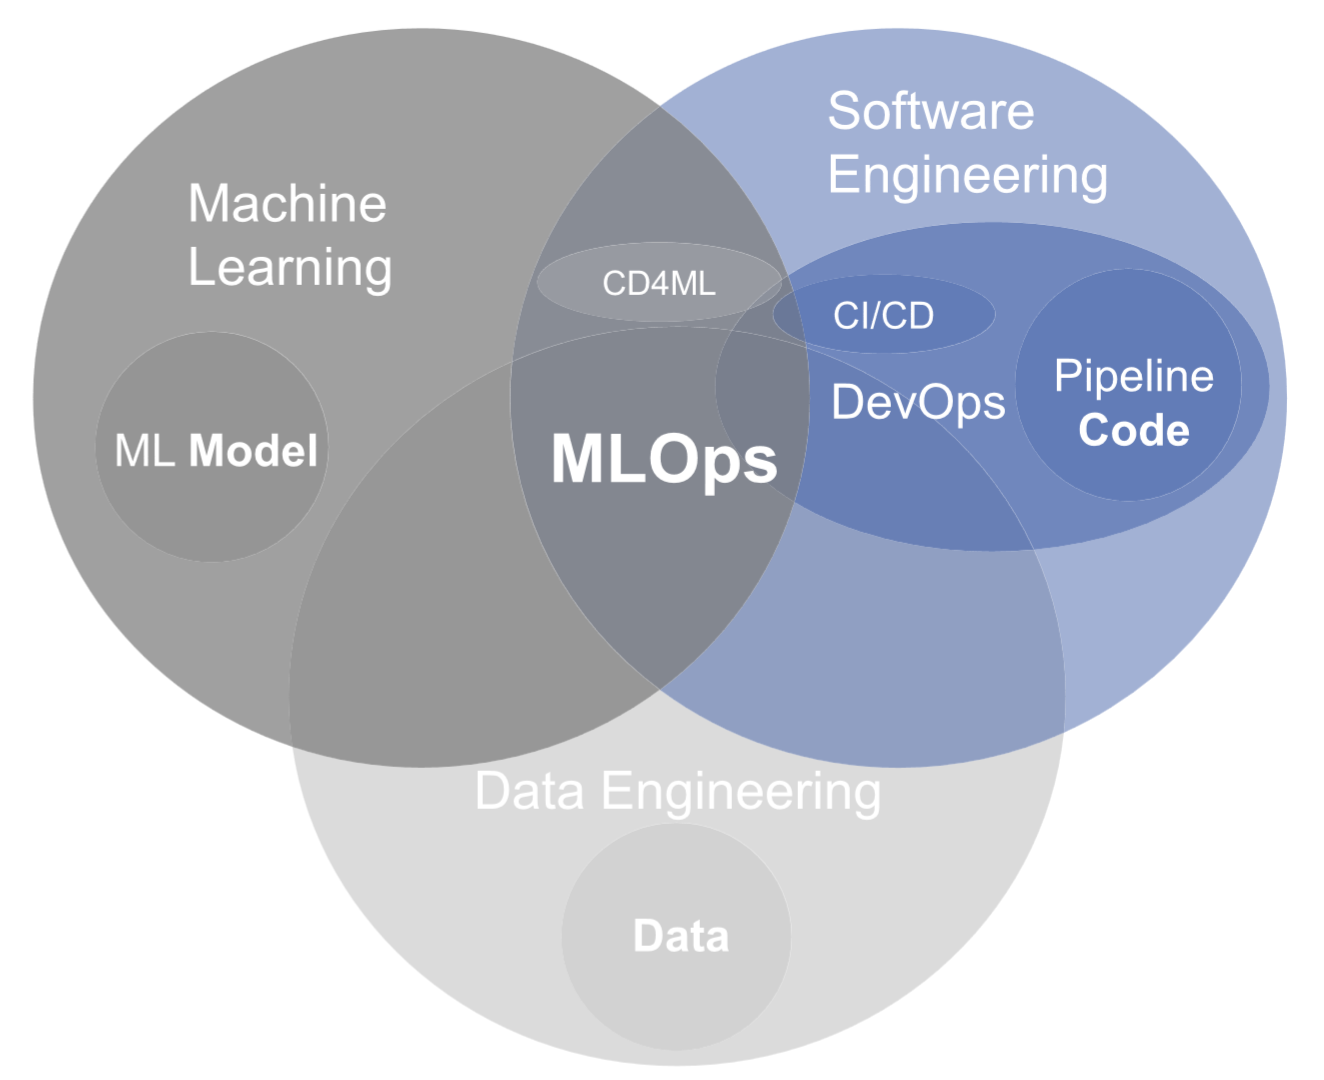
\includegraphics[width=\textwidth]{Kreuzbergeretal_fig5.png}
\end{column}
\begin{column}{.15\textwidth}
\tiny \textbf{Source:} \href{https://ieeexplore.ieee.org/abstract/document/10081336}{Kreuzberger, D., K\"uhl, N., \& Hirschl, S. (2023). Machine learning operations (mlops): Overview, definition, and architecture. IEEE access, 11, 31866-31879.}
\end{column}
\end{columns}
\end{frame}


\begin{frame}{Model Development Lifecycle}
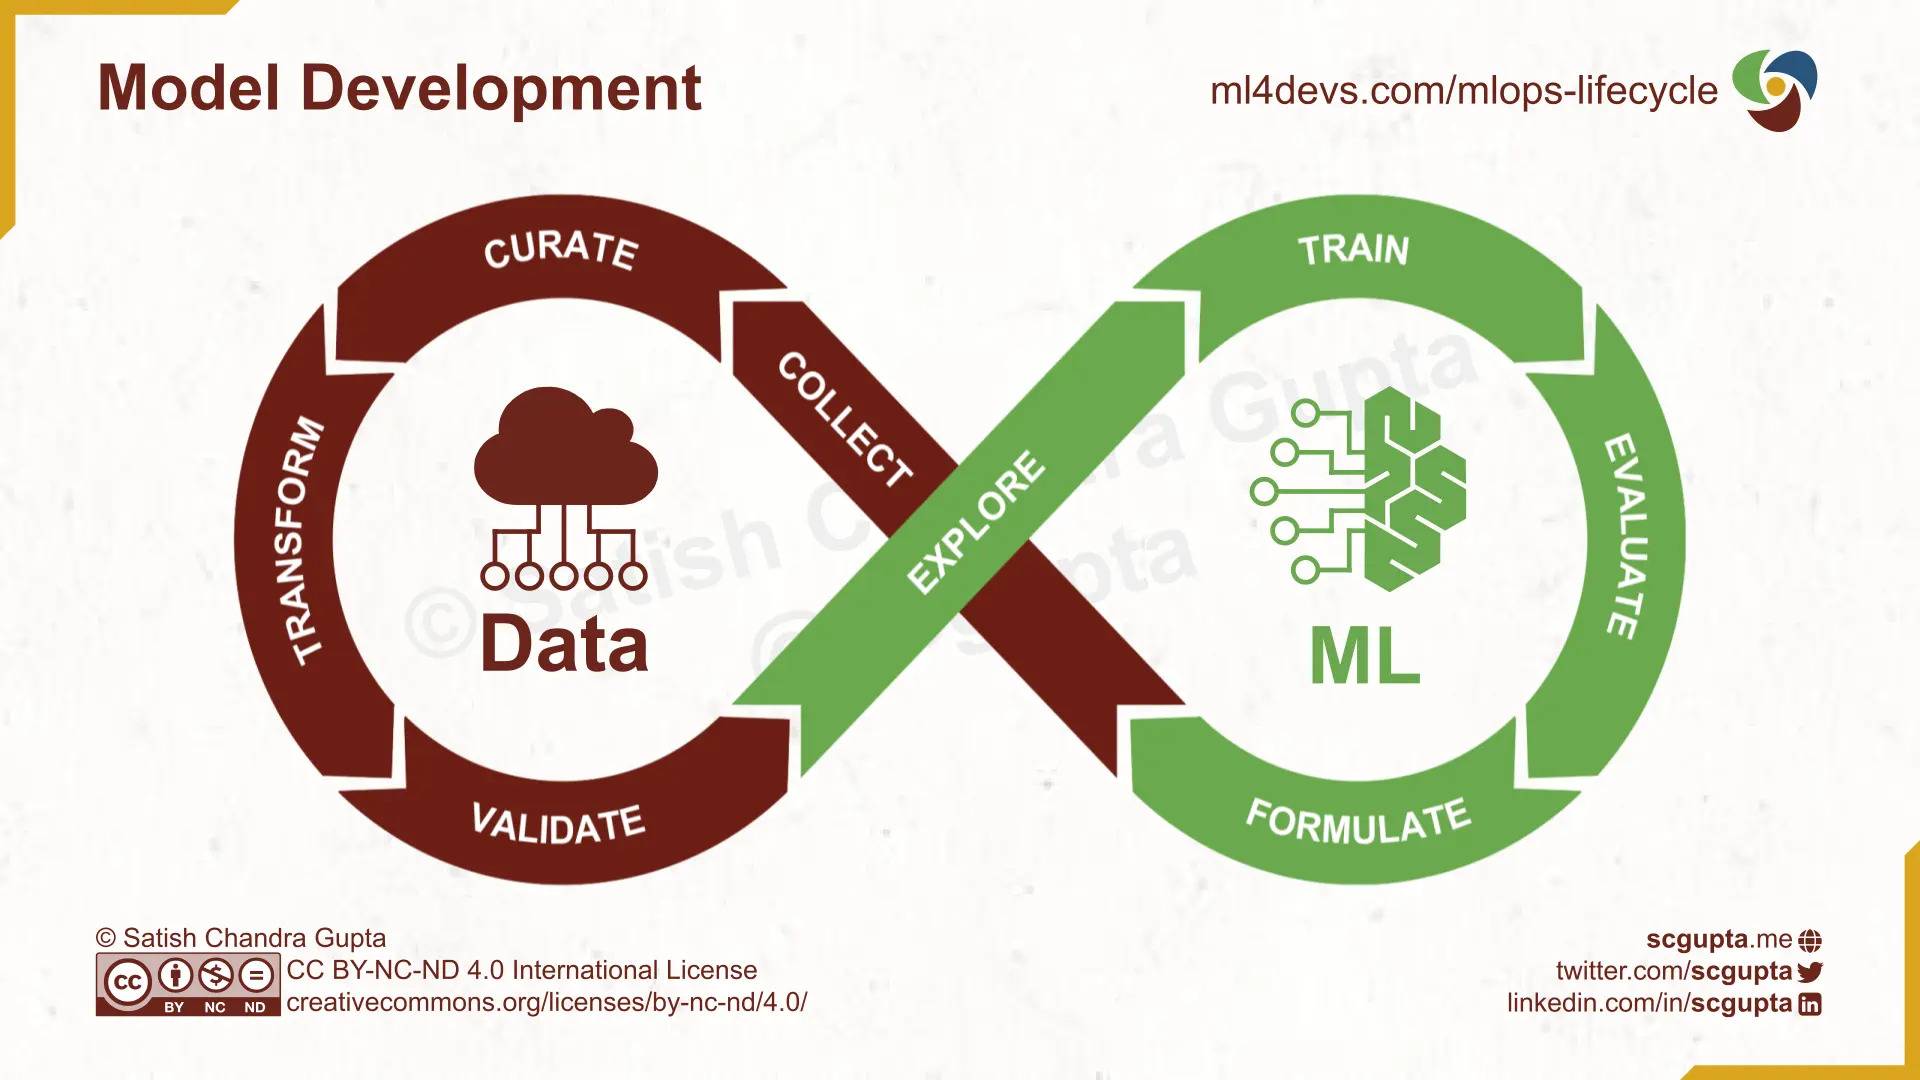
\includegraphics[width=\textwidth]{mlmodel.jpeg}
\end{frame}

\begin{frame}{Software Development Lifecycle}
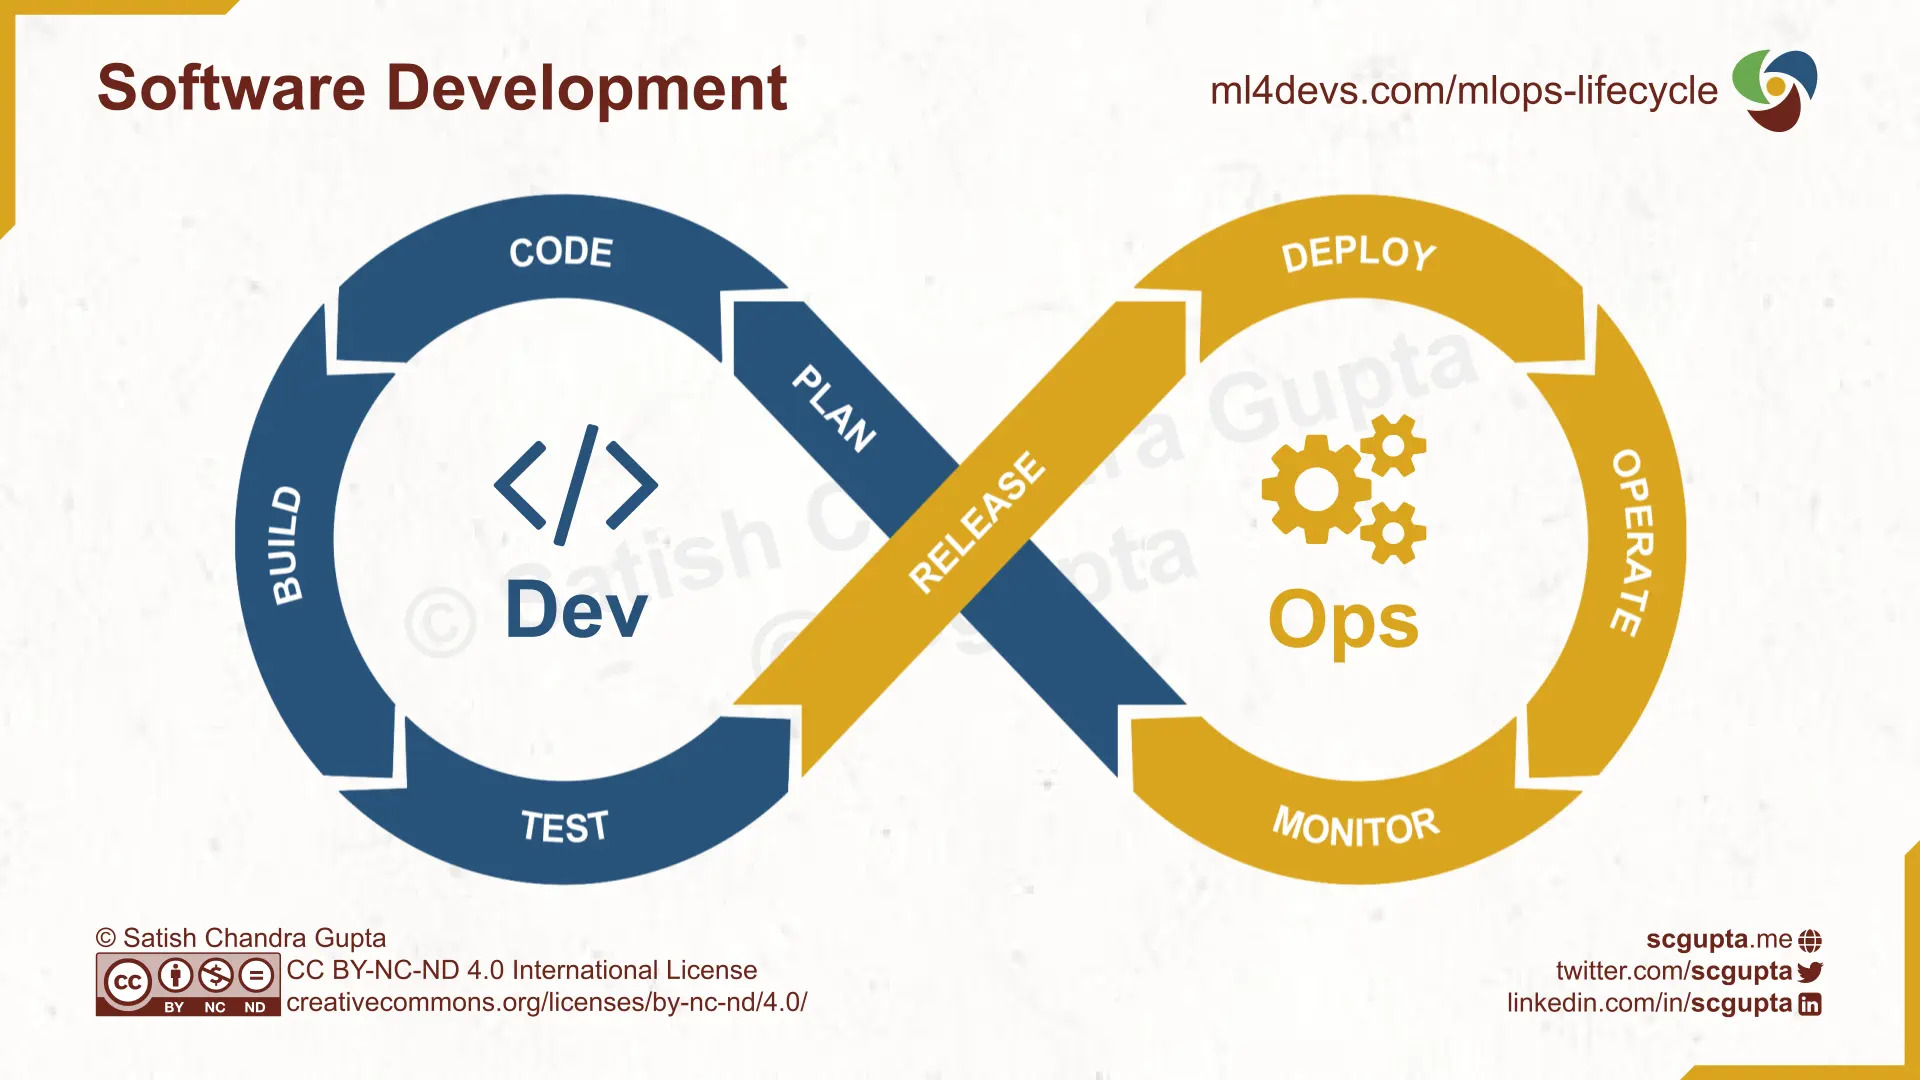
\includegraphics[width=\textwidth]{devopsmodel.jpeg}
\end{frame}

%\begin{frame}{ML Lifecycle}
%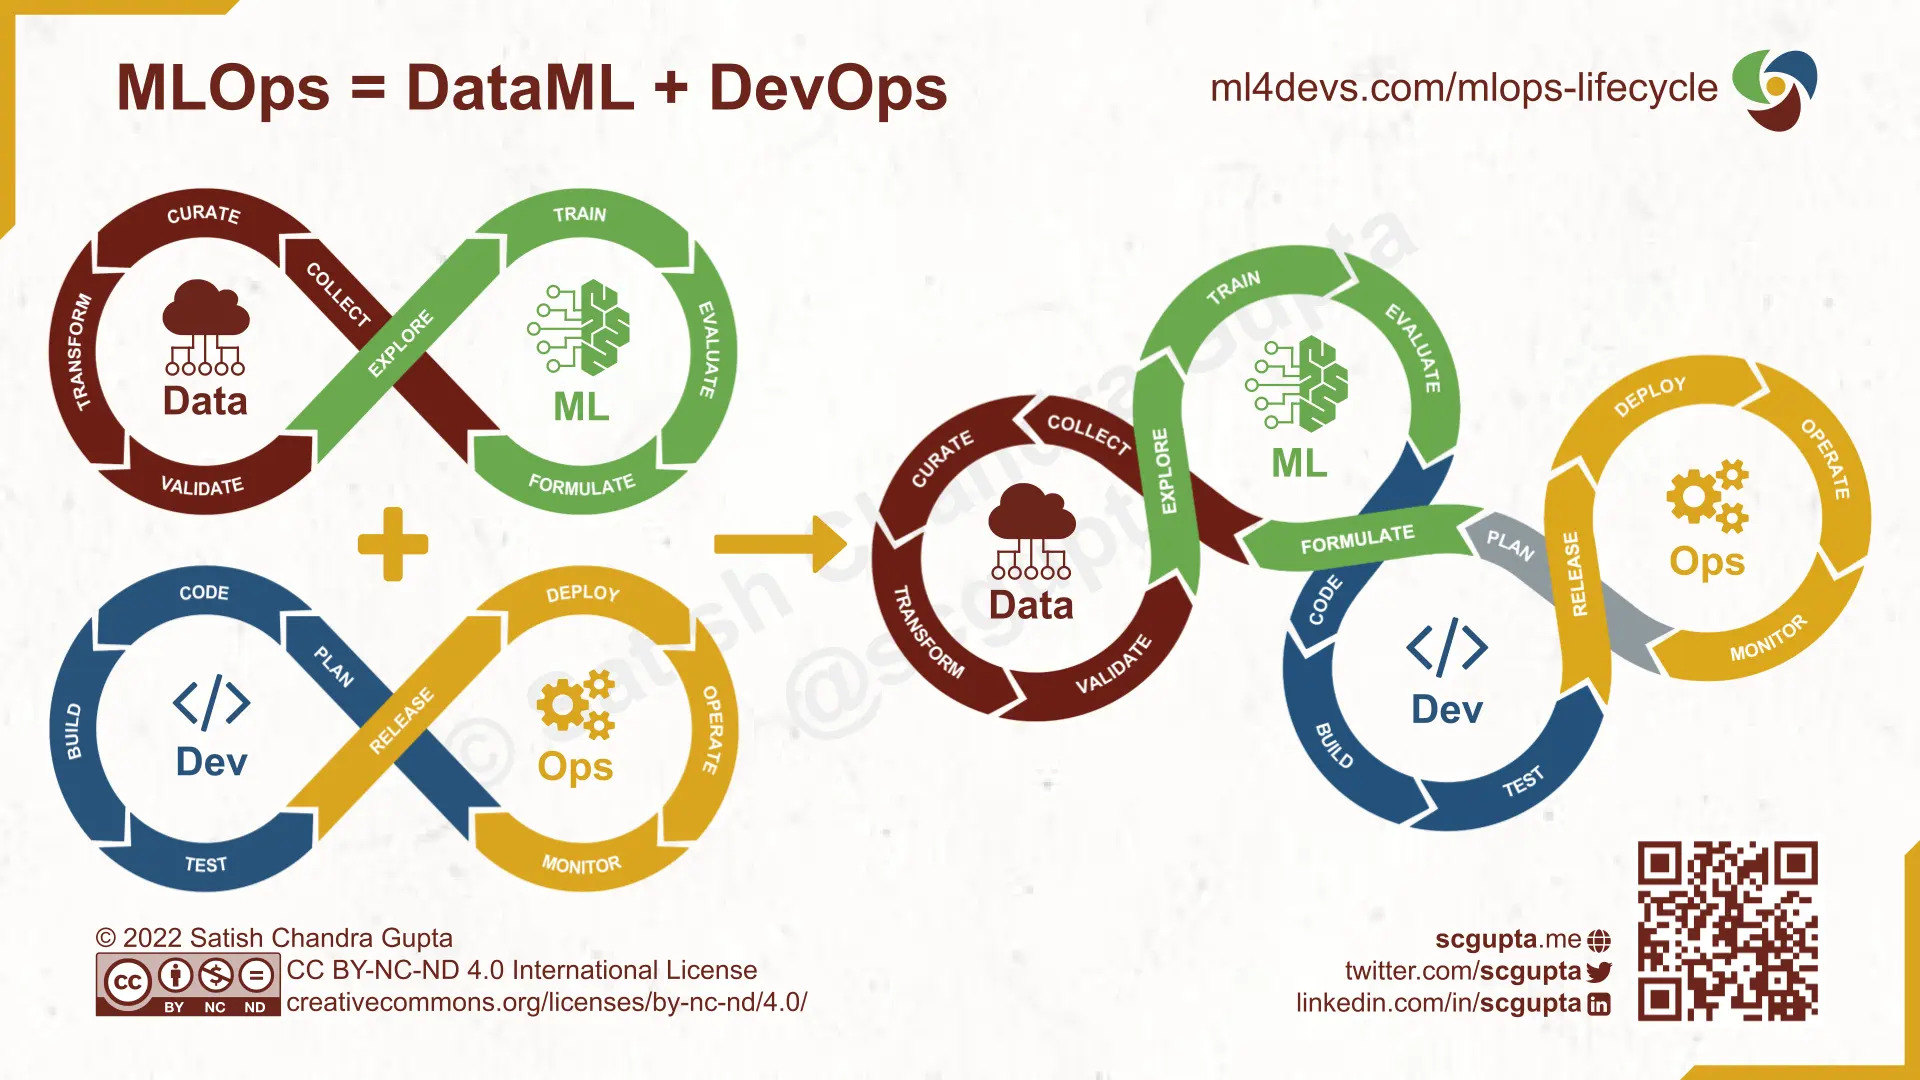
\includegraphics[width=\textwidth]{mlops.jpeg}
%\end{frame}

\begin{frame}{MLOps Lifecycle}
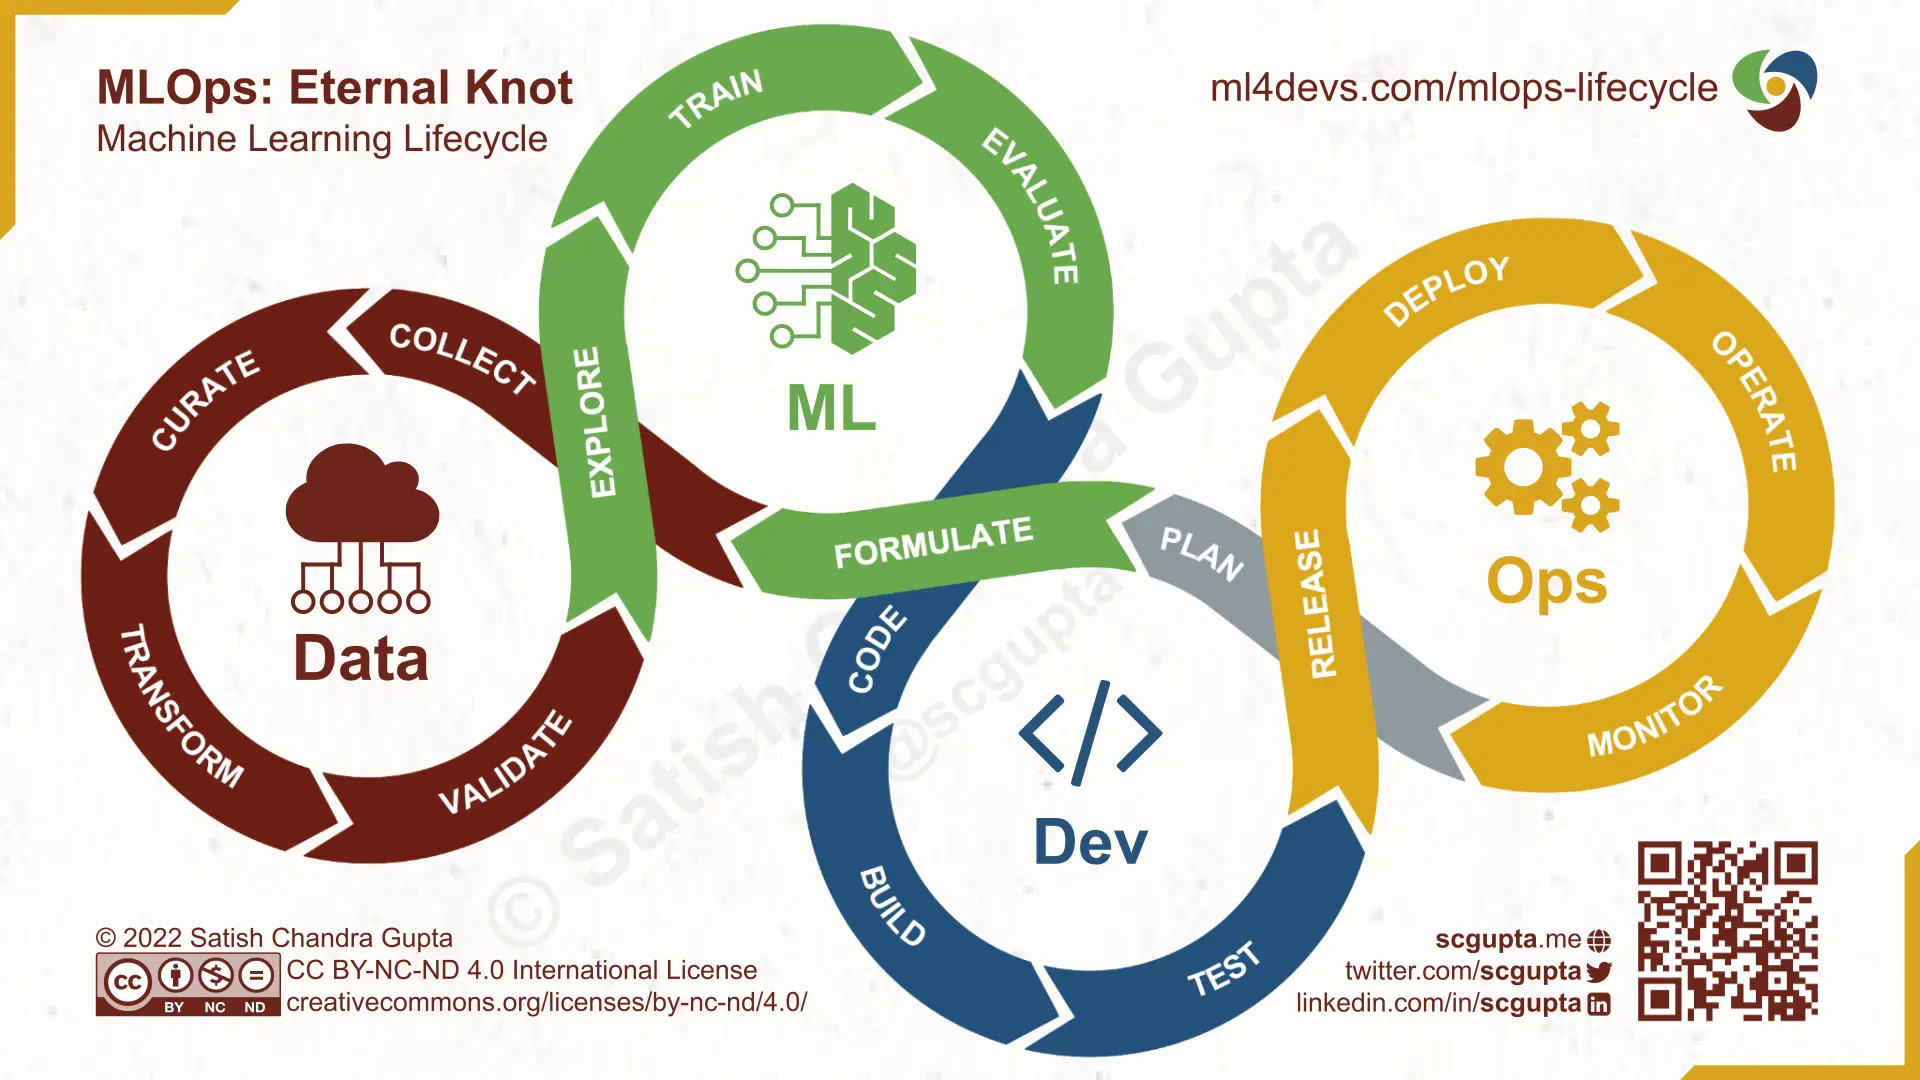
\includegraphics[width=\textwidth]{mlops2.jpeg}
\end{frame}


\begin{frame}{MLOps Participants}
\begin{itemize}
  \item Subject matter experts
  \begin{itemize}
  \footnotesize
     \item Provide business questions, goals and KPIs for models
     \item Evaluate model performance against business needs
  \end{itemize}
  \item Data scientists
  \begin{itemize}
  \footnotesize
     \item Develop and evaluate models
     \item Deliver operationalizable models
  \end{itemize}
  \item Data engineers
  \begin{itemize}
  \footnotesize
      \item Optimize retrieval and use of data
  \end{itemize}
  \item Software engineers
  \begin{itemize}
  \footnotesize
      \item Integrate models into applications
  \end{itemize}
  \item DevOps engineers
  \begin{itemize}
  \footnotesize
     \item Build systems and test for security, performance, availability
     \item CI/CD
  \end{itemize}
  \item Model risk managers and model auditors
  \begin{itemize}
  \footnotesize
      \item Minimize risk and ensure compliance
  \end{itemize}
  \item ML engineer/ML architects
  \begin{itemize}
  \footnotesize
     \item Ensure scalable and flexible environment
  \end{itemize}
\end{itemize}
\end{frame}

\begin{frame}{MLOps Participants -- Overlapping Roles}
\begin{columns}
\begin{column}{.9\textwidth}
\centering
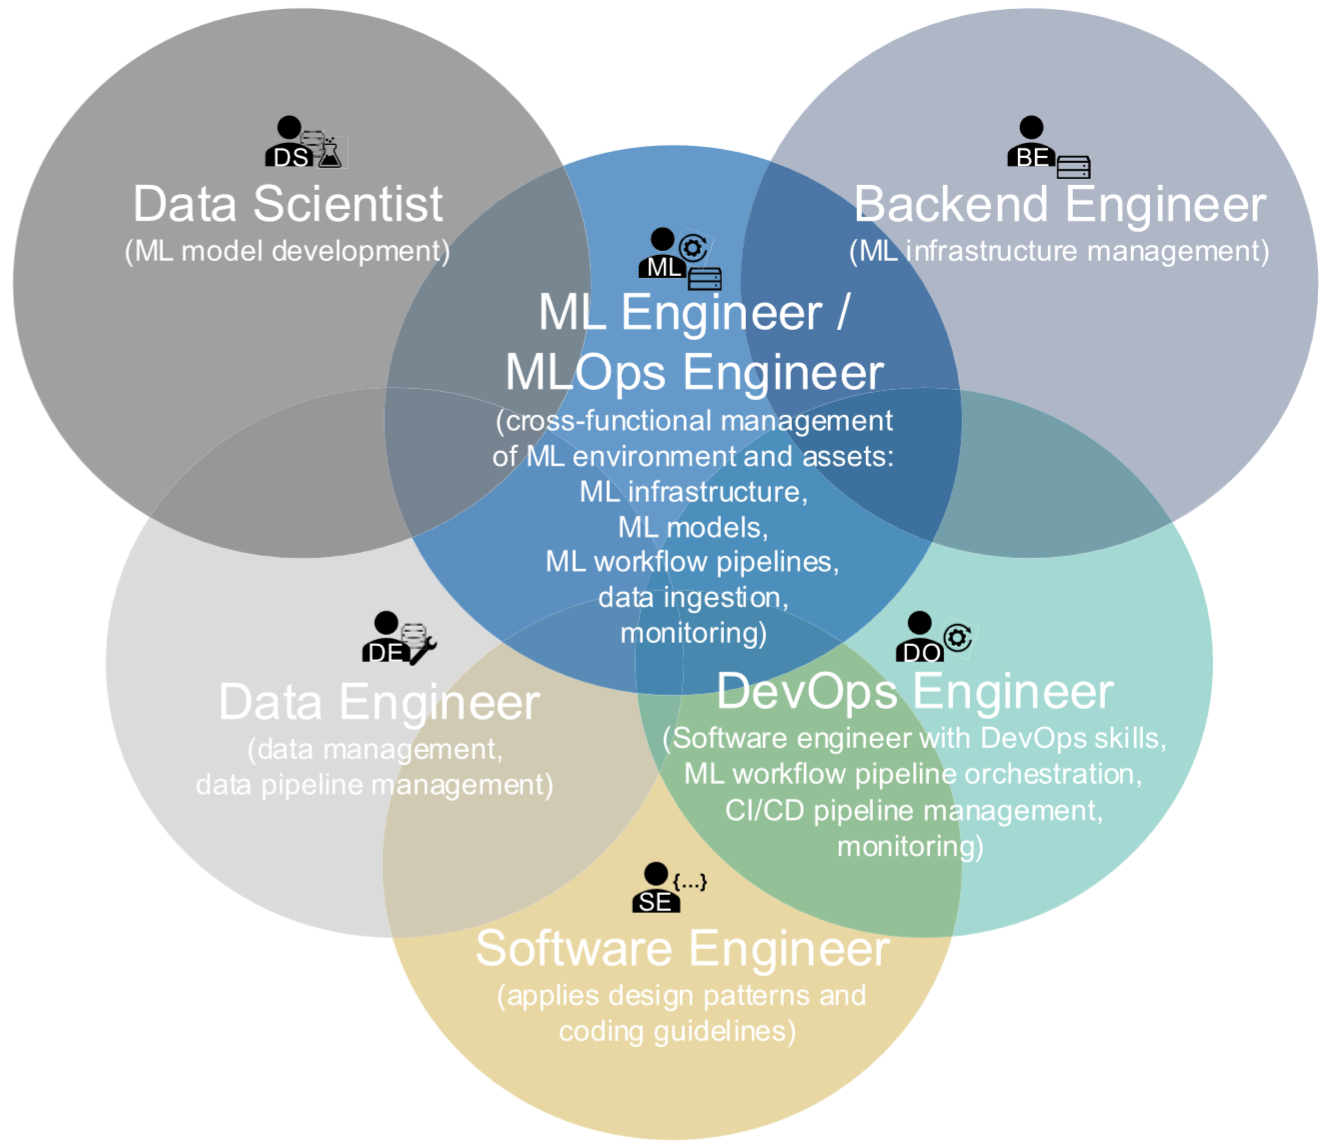
\includegraphics[width=\textwidth]{Kreuzbergeretal_fig3.png} 
\end{column}
\begin{column}{.15\textwidth}
\tiny \textbf{Source:} \href{https://ieeexplore.ieee.org/abstract/document/10081336}{Kreuzberger, D., K\"uhl, N., \& Hirschl, S. (2023). Machine learning operations (mlops): Overview, definition, and architecture. IEEE access, 11, 31866-31879.}
\end{column}
\end{columns}
\end{frame}

\begin{frame}{MLOps Participants -- Roles in MLOps lifecycle}
\begin{columns}
\begin{column}{.8\textwidth}
\centering
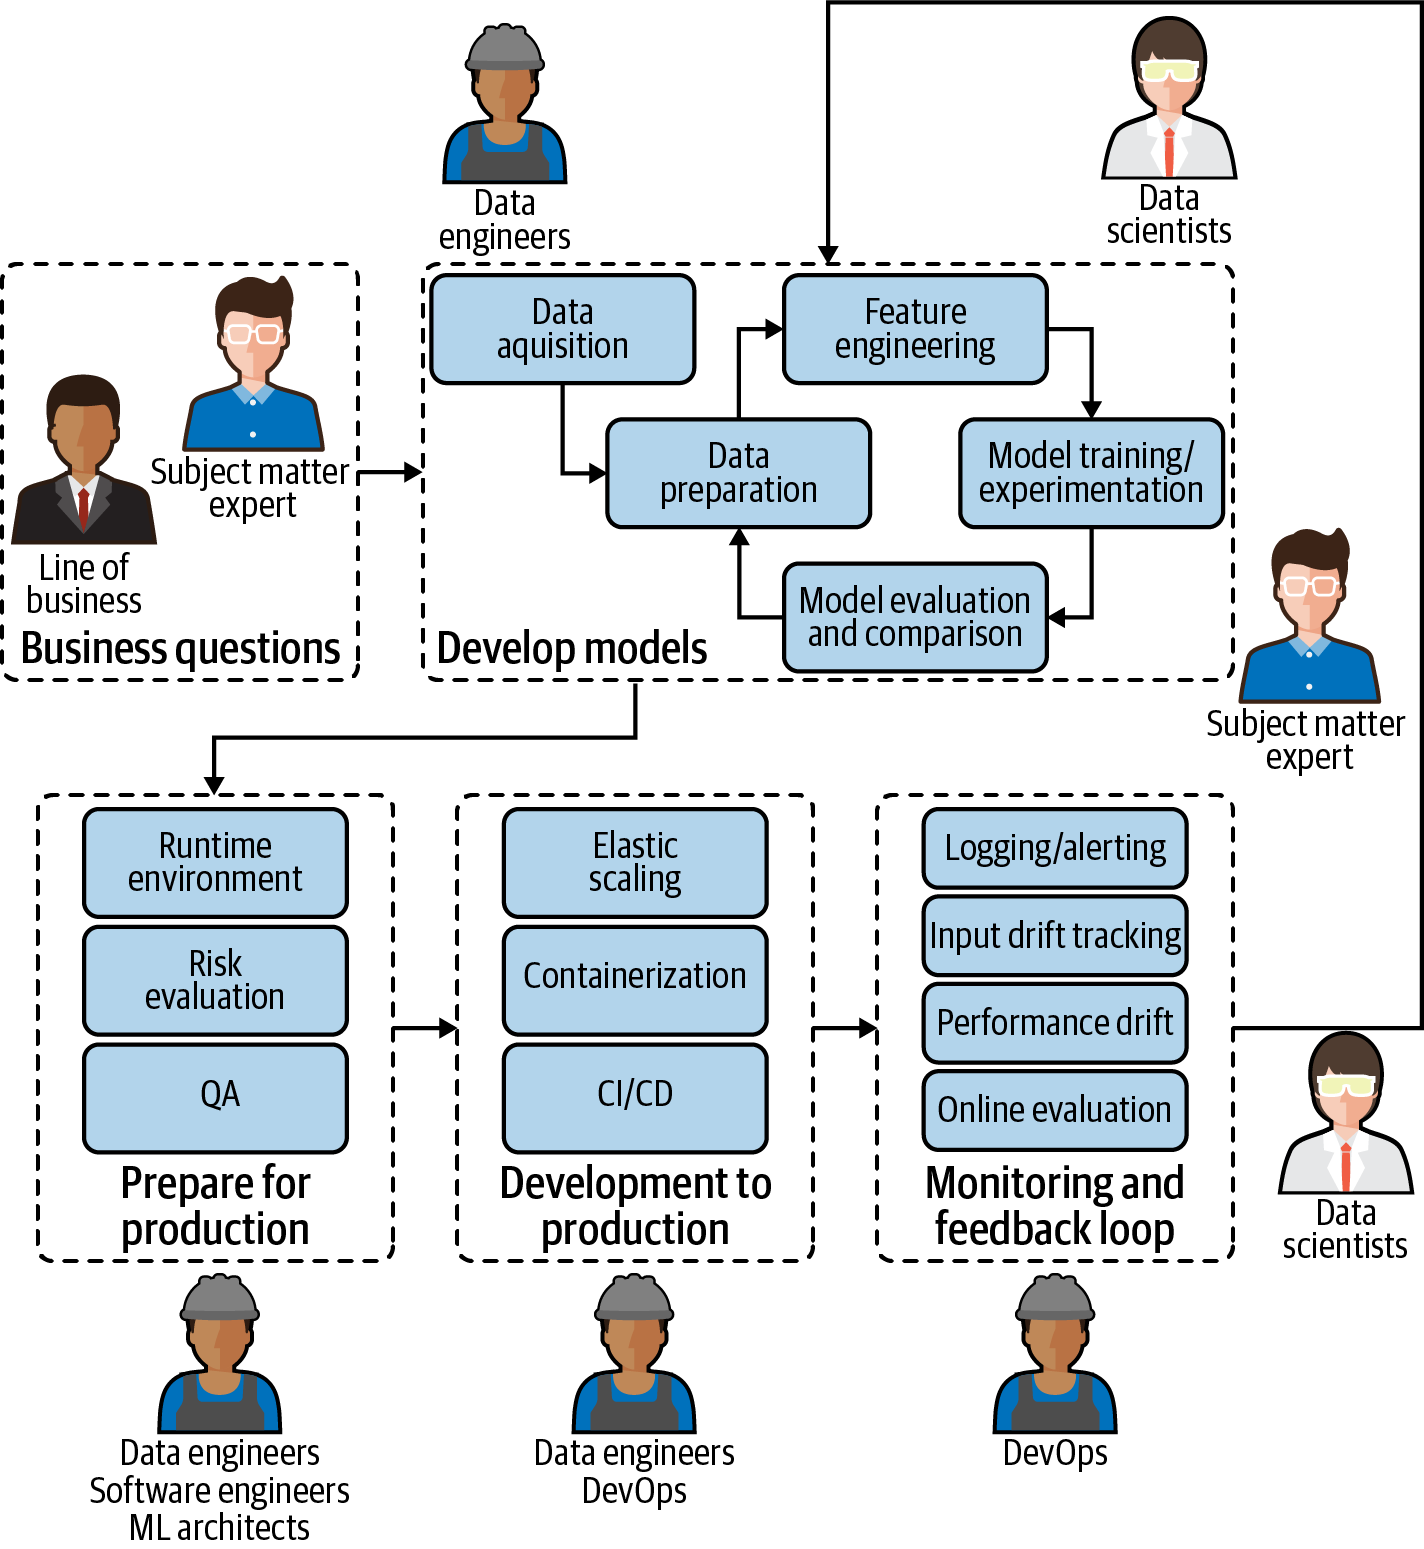
\includegraphics[height=3.25in]{imlo_0103.png}
\end{column}
\begin{column}{.2\textwidth}
\tiny \textbf{Source:} Trevail et al. (2020), Figure 1-3
\end{column}
\end{columns}
\end{frame}


\begin{frame}{MLOps -- Requirements}
\begin{itemize}
   \item Subject matter experts:
   \begin{itemize}
  \footnotesize
   \item Understandability of deployed models in business terms
   \item Feedback mechanism for models
   \end{itemize}
   \item Data scientists and data engineers:
   \begin{itemize}
  \footnotesize
   \item Automated model packaging and delivery
   \item Ability to automatically test model quality
   \item Visibility into model performance (dev, stage, production)
   \item Visibility into data pipelines for each model
   \end{itemize}
   \item Software engineers:
   \begin{itemize}
  \footnotesize
   \item Versioning and automatic testing
   \end{itemize}
   \item DevOps engineers:
   \begin{itemize}
  \footnotesize
   \item Integration with wider DevOps strategies
   \item Seamless deployment pipeline
   \end{itemize}
\end{itemize}
\end{frame}

\begin{frame}{MLOps Requirements \small [cont'd]}
\begin{itemize}
   \item Model risk managers and model auditors:
   \begin{itemize}
  \footnotesize
   \item Automated reporting on all models (past and present), including data provenance
   \end{itemize}
   \item ML engineer/architect:
   \begin{itemize}
  \footnotesize
   \item Ability to assess and adjust infrastructure capacities
   \end{itemize}
\end{itemize}
\end{frame}

\begin{frame}{MLOps -- Tooling}
\begin{itemize}
  \item Source Code Repository
  \begin{itemize}
  \footnotesize
     \item Training, inference and application source code
     \item Versioning
     \item \emph{Examples:} GitHub, GitLab
  \end{itemize}
  \item CI/CD
  \begin{itemize}
  \footnotesize
     \item Build, test, deploy
     \item \emph{Examples:} Jenkins, GitHub actions
  \end{itemize}
  \item Workflow Orchestration
  \begin{itemize}
  \footnotesize
     \item Defines execution and artifact usage
     \item Data extraction, training, inference, deployment
     \item \emph{Examples:} Apache Airflow, AWS SageMaker Pipelines, Azure Pipelines
  \end{itemize}
  \item Feature Store
  \begin{itemize}
  \footnotesize
     \item Central storage of feature data
     \item \emph{Examples:} Google Feast, AWS Feature Store, Tecton.ai
  \end{itemize}
  \item Model Training Infrastructure
  \begin{itemize}
  \footnotesize
     \item CPU and GPU for training
  \end{itemize}
\end{itemize}
\end{frame}

\begin{frame}{MLOps -- Tooling \small [cont'd]}
\begin{itemize}
  \item Model Registry
  \begin{itemize}
  \footnotesize
      \item Store trained model and metadata
      \item Versioning
      \item \emph{Examples:} MLflow, AWS SageMaker Model Registry, Azure ML Model Registry
  \end{itemize}
  \item ML Metadata Stores
  \begin{itemize}
  \footnotesize
     \item ML Pipeline execution, model training, model lineage, etc.
     \item \emph{Examples:} MLFlow
  \end{itemize}
  \item Model Serving
  \begin{itemize}
  \footnotesize
     \item Online inference, real-time predictions
     \item \emph{Examples:} Flask, TensorFlow Serving, AWS SageMaker Endpoints
  \end{itemize}
  \item Monitoring
  \begin{itemize}
  \footnotesize
     \item Performance monitoring
     \item Input drift detection
     \item \emph{Examples:} TensorBoard, AWS SageMaker model monitor
  \end{itemize}
\end{itemize}
\end{frame}

\begin{frame}{MLOps Tooling \small [cont'd]}
\centering
\large Commercial Offerings

\href{https://mattturck.com/wp-content/uploads/2021/12/2021-MAD-Landscape-v3.pdf}{
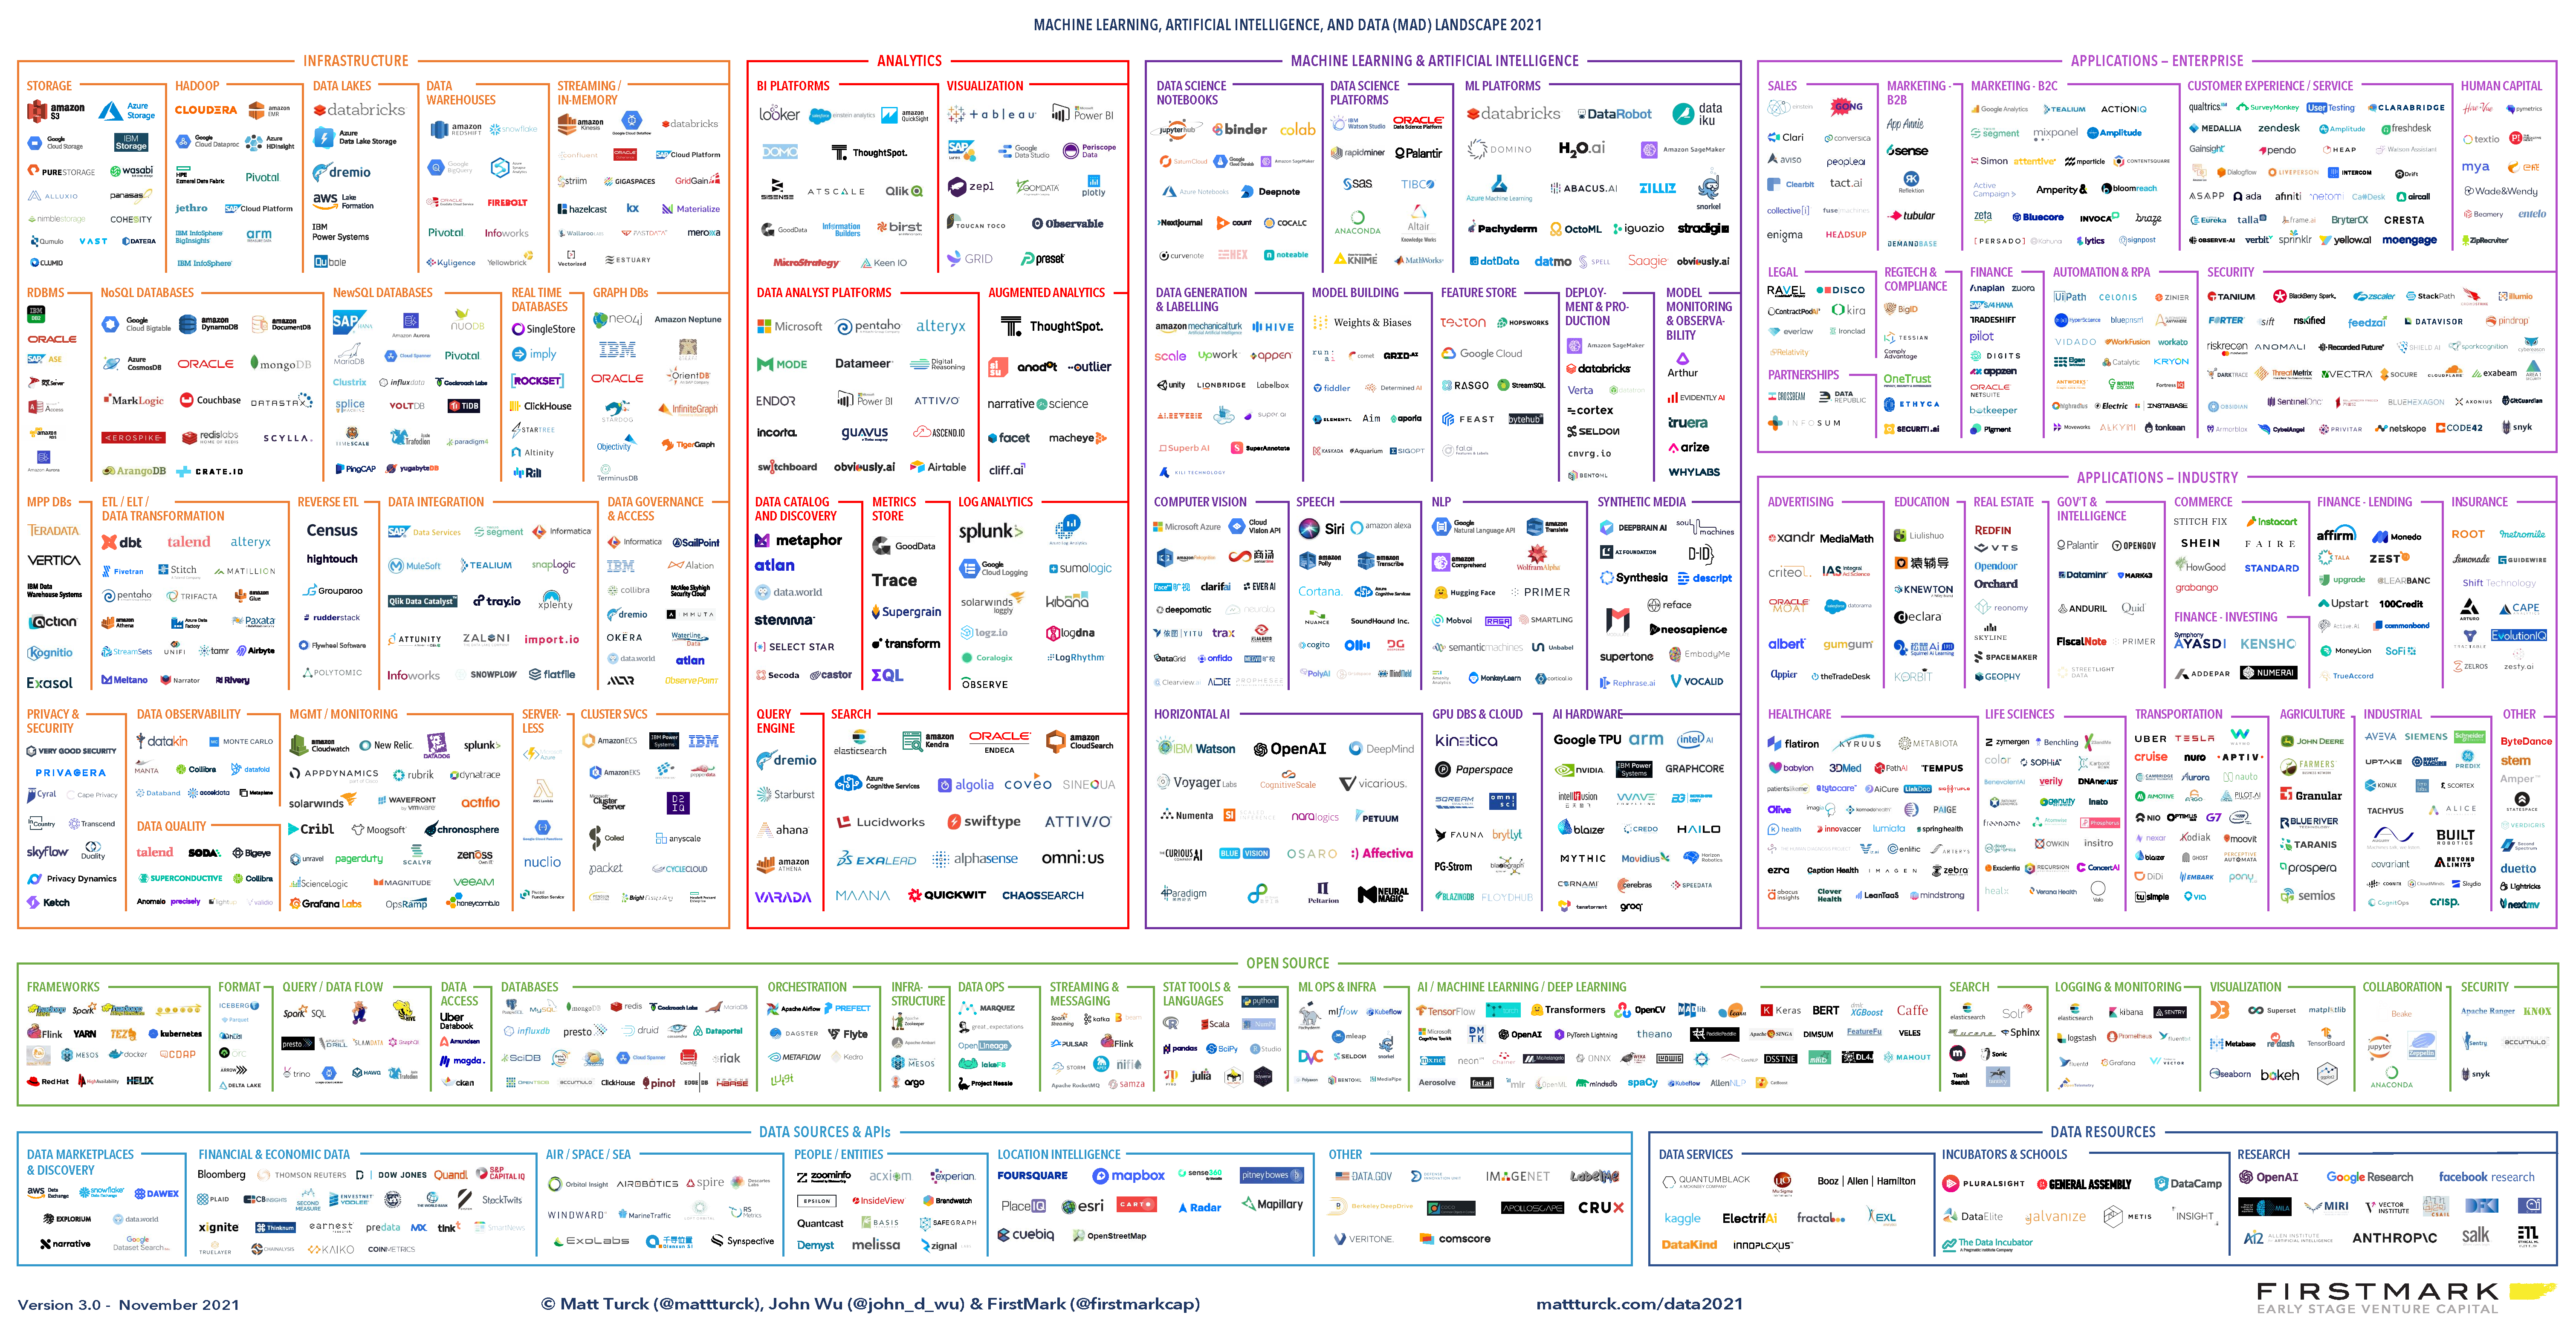
\includegraphics[width=\textwidth]{2021-MAD-Landscape-v3.pdf}} \\

\scriptsize Source: Turck, Matt. \textit{Red Hot -- The 2021 Machine Learning, AI and Data (MAD) Landscape}. September 28, 2021. \url{https://mattturck.com/data2021/} (last accessed July 22, 2024)
\end{frame}

\begin{frame}{MLOps Lifecycle}
\centering

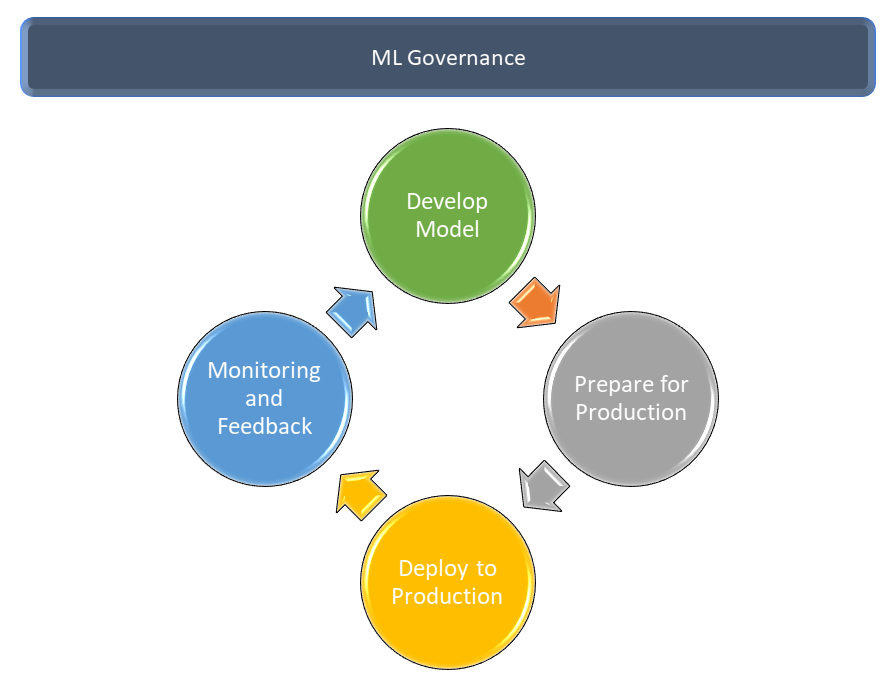
\includegraphics[height=3.25in]{graphics2.png} \\
\end{frame}


\begin{frame}{Develop Models}
\centering
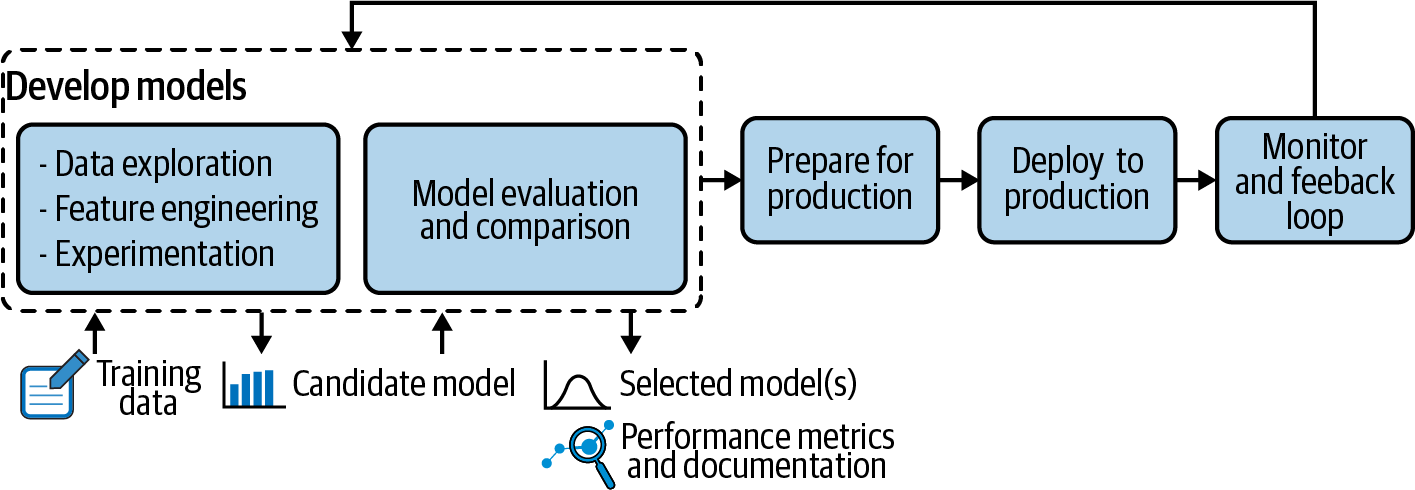
\includegraphics[width=\textwidth]{imlo_0401.png} \\

\vspace{\baselineskip}
\scriptsize Source: Treveil et al. (2020), Figure 4-1
\end{frame}

\begin{frame}{Develop Models \small [cont'd]}
\begin{block}{Data}
\begin{itemize}
   \item What data are available? What is the quality of that data?
   \item Can the data legally be used for this purpose? What are the terms of use of the data?
   \item How can the data be accessed?
   \item What features can be created by combining data sets?
   \item Must the data be redacted or anonymized?
   \item Are there features that cannot be used legally (age, gender, race, etc.)?
   \item Is the data representative of minority classes/populations?
\end{itemize}
\end{block}
\begin{block}{Automation and Tools}
\begin{itemize}
   \item ETL Pipelines (extraction from source)
   \item Data Lakes (centralized storage)
   \item Feature Stores (engineered features)
\end{itemize}
\end{block}
\end{frame}

\begin{frame}{Develop Models \small [cont'd]}
\begin{block}{Model Training}
\begin{itemize}
   \item What are appropriate evaluation metrics?
   \item Is the model performance acceptable for sub-populations?
   \item Does the model need to be interpretable or explainable?
   \item Are the model outcomes fair?
\end{itemize}
\end{block}
\begin{block}{Automation and Tools}
\begin{itemize}
   \item Model registries and repositories (weights, biases, hyperparameters, random seeds, results, etc.)
   \item Container makefiles and container registries (fixing software versions and environment)
   \item Feature Stores (training and test data versioning and update processes)
\end{itemize}
\end{block}
\end{frame}

\begin{frame}{Prepare for Production}
\centering
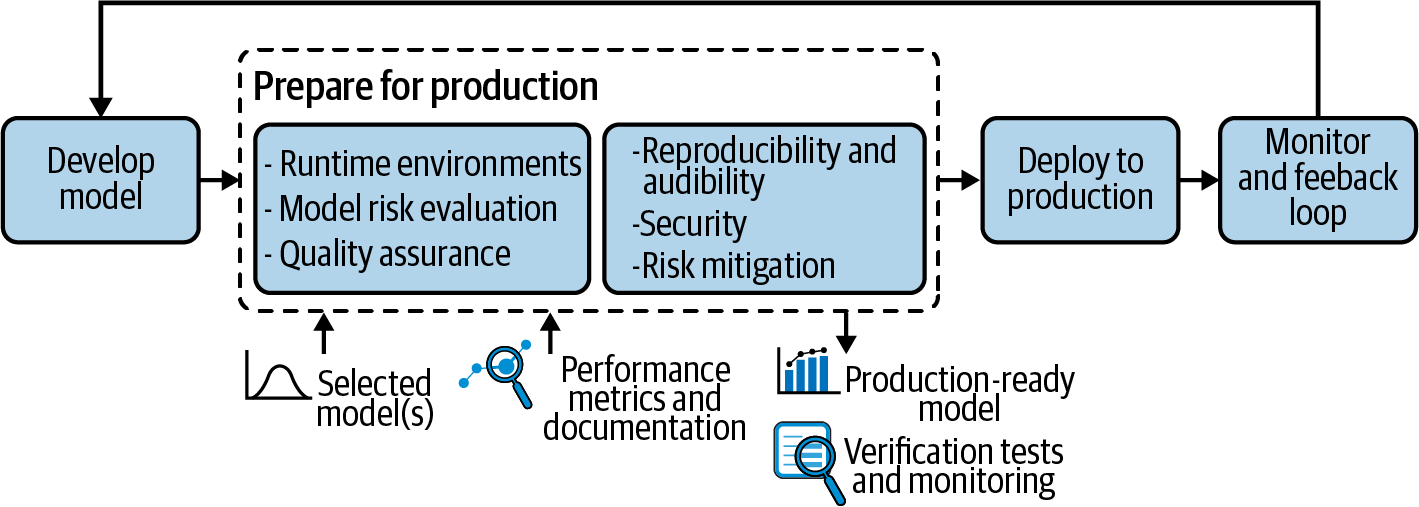
\includegraphics[width=\textwidth]{imlo_0501.png} \\

\vspace{\baselineskip}
\scriptsize Source: Treveil et al. (2020), Figure 5-1
\end{frame}

\begin{frame}{Prepare for Production \small [cont'd]}
\begin{block}{Technical Questions}
\begin{itemize}
   \item What is the runtime environment? (e.g. Flask containers, Tensorflow Serving, Kubernetes Clusters, Edge Devices, JavaScript)
   \item Does the model need to be adapted? (e.g. transformation, quantization, pruning)
   \item How are data features accessed or provided?
\end{itemize}
\end{block}
\begin{block}{Risk Assessment Questions}
\begin{itemize}
    \item What if the model acts in the worst possible way?
    \item What if a client extracts training data or model details?
    \item What are financial, business, legal, and reputational risks?
\end{itemize}
\end{block}
\end{frame}

\begin{frame}{Prepare for Production \small [cont'd]}
\begin{block}{Sources of Risk}
\begin{itemize}
   \item Errors in model design or training (incl. data prep)
   \item Errors in runtime environment
   \item Data quality problems
   \item Differences btw training \& production data (''input drift'')
   \item Abuse of model or misuse of outputs
   \item Adversarial attacks
   \item Legal risk from training data use or model results
   \item Reputational risk
\end{itemize}
\end{block}
\end{frame}

\begin{frame}{Prepare for Production \small [cont'd]}
\begin{block}{Risk Mitigation}
\begin{itemize}
   \item Shadow testing
   \item Progressive rollouts
   \item Continuous logging and monitoring
   \item Input and output checks
   \item Failover to simpler model
   \item Periodic retraining
\end{itemize}
\end{block}
\end{frame}

\begin{frame}{Prepare for Production \small [cont'd]}
\begin{block}{Automation and Tools}
\begin{itemize}
   \item Continuous integration and automated testing
   \item Model registries to document artifact
   \begin{itemize}
      \item Input data sources and provenance
      \item Model assumptions
      \item Software dependencies
      \item Test results (incl. explanations and bias evaluation)
      \item Training and test logs
   \end{itemize}
\end{itemize}
\end{block}
\end{frame}   

\begin{frame}{Deploy to Production}
\centering
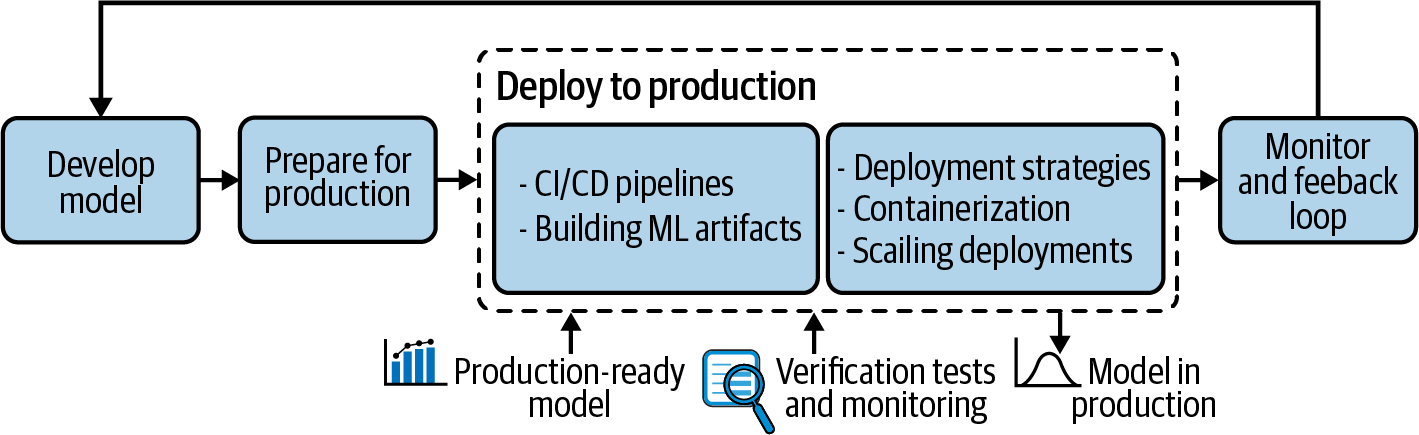
\includegraphics[width=\textwidth]{imlo_0601.png} \\

\vspace{\baselineskip}
\scriptsize Source: Treveil et al. (2020), Figure 6-1
\end{frame}

\begin{frame}{Deploy to Production \small [cont'd]}
\large Automated CI/CD Pipeline \normalsize \\

\begin{enumerate}
\item Build model
\begin{enumerate}
   \item Build model artifacts (model code, configuration, data, trained model, environment, documentation, test code and test data)
   \item Archive and register model
   \item Basic checks
   \item Evaluate bias and interpretability 
\end{enumerate}
\item Deploy to test environment
\begin{enumerate}
    \item Evaluate predictive performance
    \item Evaluate computational performance
\end{enumerate}
\item Deploy to production environment
\begin{enumerate}
   \item Limited deployment (parallel or ''canary'')
   \item Full deployment
\end{enumerate}
\end{enumerate} 

\vspace{\baselineskip}
\tiny Adapted from Trevail et al. (2020) (pg. 74, 75)
\end{frame}

\begin{frame}{Deploy to Production}
\begin{block}{Scalability and Reliability} 
\begin{itemize}
   \item Deployment targets (models to servers)
   \item Automatic Workload balancing
   \item Automatic Failover (detection, reprovisioning)
   \item Model upgrades
\end{itemize}
\end{block}
\begin{block}{Maintenance}
\begin{itemize}
   \item Continuous Resource monitoring
   \item Continuous Health checks
   \item Continuous ML metrics monitoring
\end{itemize}
\end{block}
\end{frame}

\begin{frame}{Deploy to Production}
\begin{block}{Automation and Tools}
\begin{itemize}
   \item Source code repositories (e.g. GitHub)
   \item Continuous integration (e.g. Jenkins)
   \item Model registries (e.g. MLflow)
   \item Model serving (e.g. Flask, Tensorflow Serving) 
   \item Log data storage and analysis
\end{itemize}
\end{block}
\end{frame}

%\begin{frame}{Detailed ML Activities}
%\begin{columns}
%\begin{column}{.9\textwidth}
%\centering
%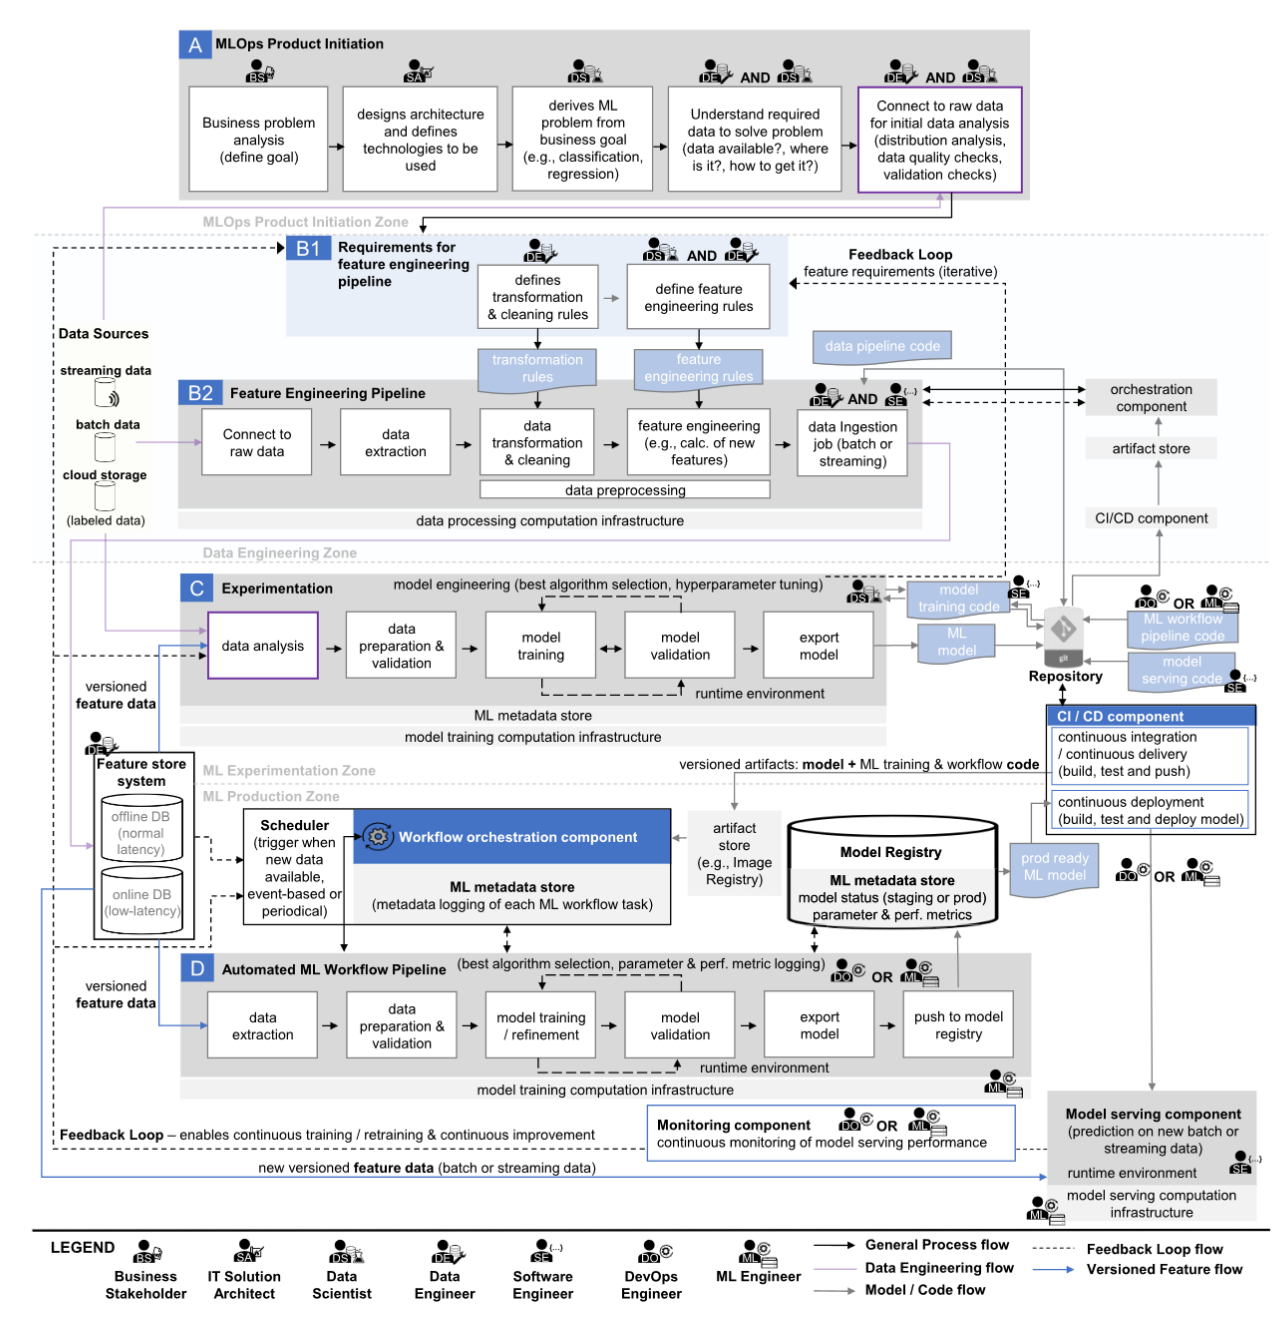
\includegraphics[height=3.25in]{Kreuzbergeretal_fig4.png} 
%\end{column}
%\begin{column}{.15\textwidth}
%\tiny \textbf{Source:} Kreuzberger, D., K\"uhl, N., \& Hirschl, S. (2023). Machine learning operations (mlops): Overview, definition, and architecture. IEEE access, 11, 31866-31879.
%\end{column}
%\end{columns}
%\end{frame}

\begin{frame}{Deployment Options}
\begin{itemize}
   \item Microservice (e.g. Flask)
   \item Tensorflow TFX and Tensorflow Serving 
   \item Tensorflow JS (for browser deployment)
   \item Tensorflow Lite (for edge devices and mobile apps)
\end{itemize}
\end{frame}

\begin{frame}[fragile]{Flask Example -- Step 1: Create a Trained Model} 

Complete file is available on \href{https://github.com/jevermann/busi4720-mlops/blob/main/train_model.py}{GitHub}. \\

Define the model and train it:
\begin{pythoncode}
import keras.utils
import pandas as pd
import tensorflow as tf
import tensorflowjs as tfjs

keras.utils.set_random_seed(42)
boston_data = \
 pd.read_csv("https://evermann.ca/busi4720/boston.csv")

boston_features = boston_data[['rm', 'tax', 'age']]
boston_labels = boston_data['medv']

# Linear regression model
norm_boston_model=keras.models.Sequential([
    keras.layers.Input(shape=(3,), dtype=tf.float32),
    keras.layers.Dense(1, activation=None) ])
\end{pythoncode}
\end{frame}

\begin{frame}[fragile]{Flask Example \small [cont'd]}
Fit the model and save it:
\begin{pythoncode}
stop_callback = keras.callbacks.EarlyStopping()
norm_boston_model.compile(
    loss = tf.keras.losses.MeanSquaredError())
norm_boston_model.fit(
    boston_features, boston_labels,
    epochs=100, validation_split=0.33,
    callbacks=[stop_callback])

# Save model for use in Keras
norm_boston_model \
    .save('norm.boston.model.trained.save')
# Export model for use in TF Serving
norm_boston_model \
    .export('norm.boston.model.trained.export')
# Convert model for use in TFJS
tfjs.converters.save_keras_model(norm_boston_model, \
    'norm.boston.model.trained.tjfs')
\end{pythoncode}
\end{frame}

\begin{frame}[fragile]{Flask Example -- Step 2: Serve the Model}
Complete file is available on \href{https://github.com/jevermann/busi4720-mlops/blob/main/flask_deploy.py}{GitHub}. \\

Load the model for prediction:
\begin{pythoncode}
import keras
import flask
from flask import request
import pandas as pd

# Load the trained model
norm_boston_model = keras.saving. \
    load_model('norm.boston.model.trained.save')

# A predict function for the model
def predict(inputs):
    return norm_boston_model. \
        predict_on_batch(inputs)[0][0]

app = flask.Flask(__name__)
\end{pythoncode}
\end{frame}

\begin{frame}[fragile]{Flask Example \small [cont'd]}

Define the URL handler and run app:
\begin{pythoncode}
@app.route("/predict_json", methods=["POST"])
def predict_json():
    reply = {}
    # TODO: Input checking goes here
    # TODO: Input logging goes here
    inputs = pd.DataFrame \
               .from_dict(request.json) \
               .transpose()
    prediction = predict(inputs)
    # TODO: Output checking goes here
    # TODO: Output logging goes here
    reply["prediction"] = str(prediction)
    reply["success"] = True
    return flask.jsonify(reply)
    
app.run()
\end{pythoncode}
\end{frame}

\begin{frame}[fragile]{Flask Example -- Step 3: Access the Service}
Complete file is available on \href{https://github.com/jevermann/busi4720-mlops/blob/main/json_demo.sh}{GitHub}. \\

Access the prediction with JSON POST request:
\begin{bashcode}
#!/usr/bin/bash
curl -X POST \
     -H "Content-Type: application/json" \
     --data '[6, 250, 66.5]' \
     http://localhost:5000/predict_json
\end{bashcode}
\end{frame}

\begin{frame}[fragile]{Flask Example -- Web Forms}
Complete file is available on \href{https://github.com/jevermann/busi4720-mlops/blob/main/predict_form_async.html}{GitHub}. \\

Access using a JSON POST request from a Web Form:
\begin{htmlcode}
<!DOCTYPE html>
<html lang="en">
 <head>
  <meta charset="UTF-8">
   <title>Boston Housing Data Prediction Service</title>
   <script>
    async function predict() {
     // Get the values from the text inputs
     const rooms = 
      parseFloat(document.getElementById('rooms').value);
     const tax = 
      parseFloat(document.getElementById('tax').value);
     const age = 
      parseFloat(document.getElementById('age').value);
     // Create a JSON payload
     const payload = JSON.stringify([rooms, tax, age]);
\end{htmlcode}
\end{frame}

\begin{frame}[fragile]{Flask Example \small [cont'd]}
\begin{htmlcode}
     // Make a POST request to the server
     const response = await fetch('/predict_json', {
       method: 'POST',
       headers: {
         'Content-Type': 'application/json'
       },
       body: payload
     });
     // Parse the JSON response
     const result = await response.json();
     // Display the result
     document.getElementById('output-div').textContent
       = result.prediction;
   }
  </script>
 </head>
\end{htmlcode}
\end{frame}

\begin{frame}[fragile]{Flask Example \small [cont'd]}
\begin{htmlcode}
 <body>
  <h1>Boston Housing Data Inputs</h1>
  <form onsubmit="event.preventDefault(); predict();">
   <p>
    <label for="rooms">Number of Rooms</label>
    <input name="rooms" id="rooms" required>
   </p>
   <p>
    <label for="tax">Tax Rate per $10,000</label>
    <input name="tax" id="tax" required>
   </p>
   <p>
    <label for="age">Prop bldg older than 1940</label>
    <input name="age" id="age" required>
   </p>
   <input type="submit" value="Submit">
  </form>
  <p>Prediction is: <div id="output-div">...</div></p>
 </body>
</html>
\end{htmlcode}
\end{frame}

\begin{frame}[fragile]{Tensorflow JS Example}
Complete file is available on \href{https://github.com/jevermann/busi4720-mlops/blob/main/tjfs_demo.html}{GitHub}.
\begin{htmlcode}
<!DOCTYPE html>
<html>
 <head>
  <script src="https://cdn.jsdelivr.net/npm/\
     @tensorflow/tfjs@latest/dist/tf.min.js"></script>
  <script>
   async function predict() {
    // Load the model
    const model = await \
     tf.loadLayersModel('https://raw.githubusercontent.\
      com/jevermann/busi4720-mlops/main/model.json');
    // Get the values from the text inputs
    const rooms = 
     parseFloat(document.getElementById('rooms').value);
    const tax = 
     parseFloat(document.getElementById('tax').value);
    const age = 
     parseFloat(document.getElementById('age').value);
\end{htmlcode}
\end{frame}
\begin{frame}[fragile]{Tensorflow JS Examples \small [cont'd]}
\begin{htmlcode}
    // Package the values into a Tensor
    const inputs = tf.tensor2d([rooms, tax, age],[1, 3]);
    // Get the prediction from the model
    document.getElementById('output-div').innerText = 
     model.predict(inputs).dataSync();
   }
  </script>
 </head>
\end{htmlcode}
Remainder of the Web form as above.
\end{frame}

\begin{frame}{Monitoring and Feedback}
\centering
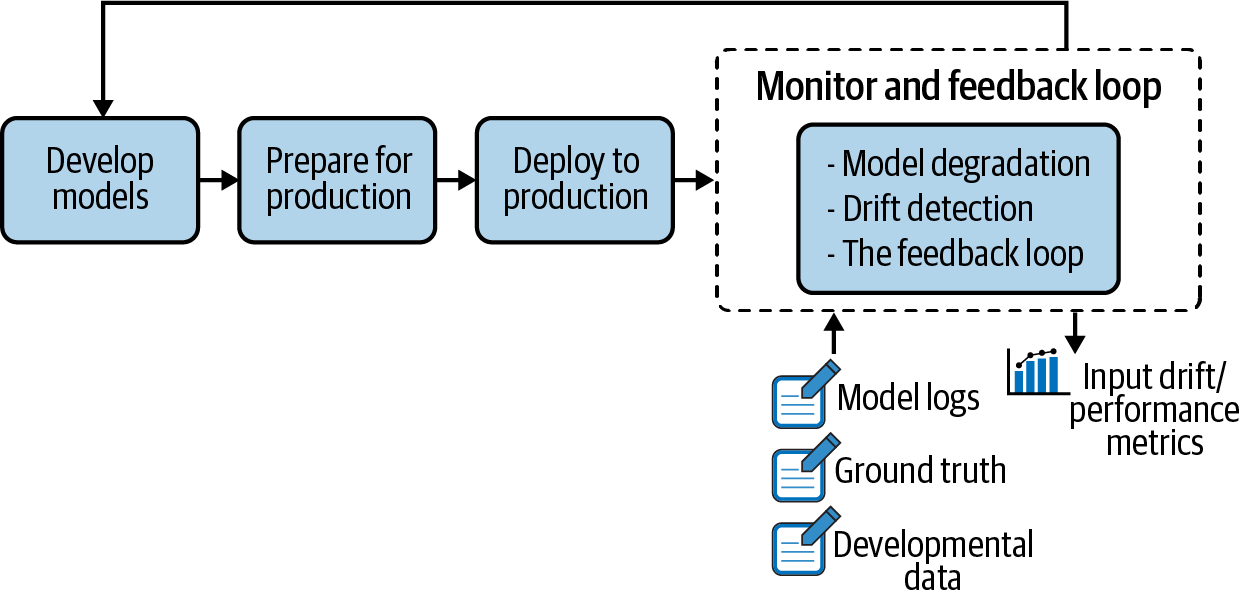
\includegraphics[width=\textwidth]{imlo_0701.png} \\

\vspace{\baselineskip}
\scriptsize Source: Treveil et al. (2020), Figure 7-1
\end{frame}

\begin{frame}{Monitoring and Feedback \small [cont'd]}
\begin{block}{Model Retraining Considerations}
\begin{itemize}
   \item Domain changes
   \item Training cost
   \item Model performance
   \item Ground truth availability
\end{itemize}
\end{block}
\begin{block}{Ground Truth for Monitoring and Retraining}
\begin{itemize}
   \item Not always immediately or imminently available (e.g. loan repayment)
   \item Ground truth and prediction are decoupled (e.g. missing or mismatched identifiers)
   \item Ground truth not available for all classes (e.g. fraud detection)
\end{itemize}
\end{block}
\end{frame}

\begin{frame}{Monitoring and Feedback \small [cont'd]}
\begin{block}{Input Drift Causes}
\begin{itemize}
   \item Selection bias
   \item Non-stationary environment
\end{itemize}
\end{block}
\begin{block}{Input Drift Detection}
\begin{itemize}
   \item Univariate statistical tests (e.g. $\chi^2$ or Kolmogorov-Smirnov)\footnote{\url{https://en.wikipedia.org/wiki/Chi-squared_test}} \footnote{\url{https://en.wikipedia.org/wiki/Kolmogorov-Smirnov_test}}
   \item Domain classifier approach (train classifier to predict old or new sample domain)
\end{itemize}
\end{block}
\end{frame}

\begin{frame}{Monitoring and Feedback \small [cont'd]}
\begin{block}{Feedback Loop Requirements}
\begin{itemize}
   \item Logging (metadata, inputs, outputs, actions taken, explanations)
   \item Model store (features, preprocessing, train and test data, algorithm, eval metrics)
   \item Online evaluation (shadow testing or A/B testing)
\end{itemize}
\end{block}
\end{frame}

\begin{frame}[fragile]{Basic Python Logging}
Complete file is available on \href{https://github.com/jevermann/busi4720-mlops/blob/main/flask_deploy_logging.py}{GitHub}. \\

Set up the logger:
\begin{pythoncode}
import logging.handlers

req_logger=logging.getLogger(model_name+'.requests')
req_logger.setLevel(logging.INFO)
req_logger.addHandler(
    logging.FileHandler(
        model_name+'.requests.log'))
# req_logger.addHandler(
#     logging.handlers.RotatingFileHandler(
#         model_name+'.requests.log',
#         maxBytes=1000000,
#         backupCount=5))
\end{pythoncode}
\end{frame}

\begin{frame}[fragile]{Basic Python Logging \small [cont'd]}
Use the logger:
\begin{pythoncode}
@app.route("/predict_json", methods=["POST"])
def predict_json():
    req_logger.info('%s TIME %s IP %s JSON %s', 
                    model_name, 
                    time.ctime(), 
                    request.remote_addr, 
                    request.json)
...
def predict_form():
    req_logger.info('%s TIME %s IP %s FORM %s',
                    model_name,
                    time.ctime(),
                    request.remote_addr,
                    request.form)
...
\end{pythoncode}
\end{frame}

\begin{frame}{Hands-On Exercise}
\begin{enumerate}
\item Download the complete file from \href{https://github.com/jevermann/busi4720-mlops/blob/main/flask_deploy_logging.py}{GitHub}. \\
\item Define a second logger that writes to a different log file
\begin{itemize}
  \item You do not need to rotate this log file
  \item The definition of the second logger is analogous to that of the request logger
\end{itemize}
\item Add logging to the \texttt{predict\_json()} and the \texttt{predict\_form()} functions to capture the time, the three inputs, and the prediction in the log.
\begin{itemize}
   \item Replace the \texttt{\# TODO: Output logging goes here} comments with your code
   \item To make the log easy to analyze, write the information in CSV format. Make sure you quote the fields that need quoting.
\end{itemize}
\end{enumerate}
\end{frame}

\begin{frame}{MLOps Governance}
\centering

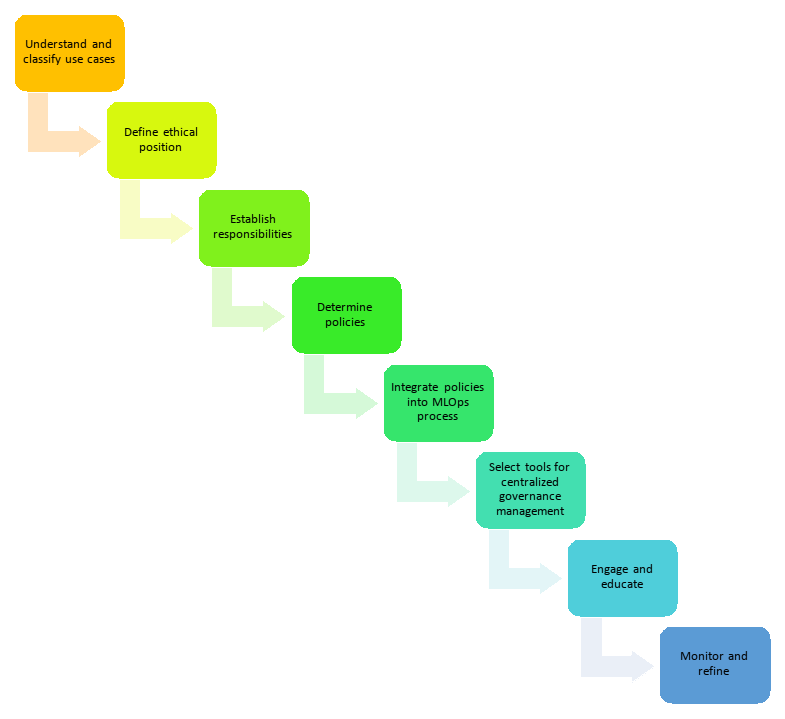
\includegraphics[height=3.25in]{governancegraphics.png}
\end{frame}

\begin{frame}{MLOps Governance}
\footnotesize
\begin{block}{1. Understand ML Uses}
\begin{itemize}
  \item Who is the consumer of the model output?
  \item What regulations and legal constraints apply?
  \item What are the legal, financial, reputational risks of errors?
  \item What is need for explainability or interpretability?
  \item What are the availability requirements?
  \item What is the model lifetime and likely rate of model decay?
\end{itemize}
\end{block}
%\end{frame}

%\begin{frame}{MLOps Governance \small [cont'd]}
%\small
\begin{block}{2. Define Ethical Position}
\begin{itemize}
  \item How important are aspects like equality, privacy, human rights, democracy, bias?
  \item How transparent should decision making be?
  \item What level of responsibility for errors will the business assume?
  \item What is the potential for deception, manipulation, exploitation?
\end{itemize}
\end{block}
\tiny Adapted from Treveil et al. (2020), Chapter 8
\end{frame}

\begin{frame}{MLOps Governance \small [cont'd]}
\footnotesize
\begin{block}{3. Establish Responsibilities (''Who will do what?'')}
\begin{itemize}
  \item Strategic, tactical, and operational
  \item Senior management sponsorship
  \item Integrate into existing governance mechanisms
\end{itemize}

\begin{columns}
\begin{column}{.8\textwidth}
\centering
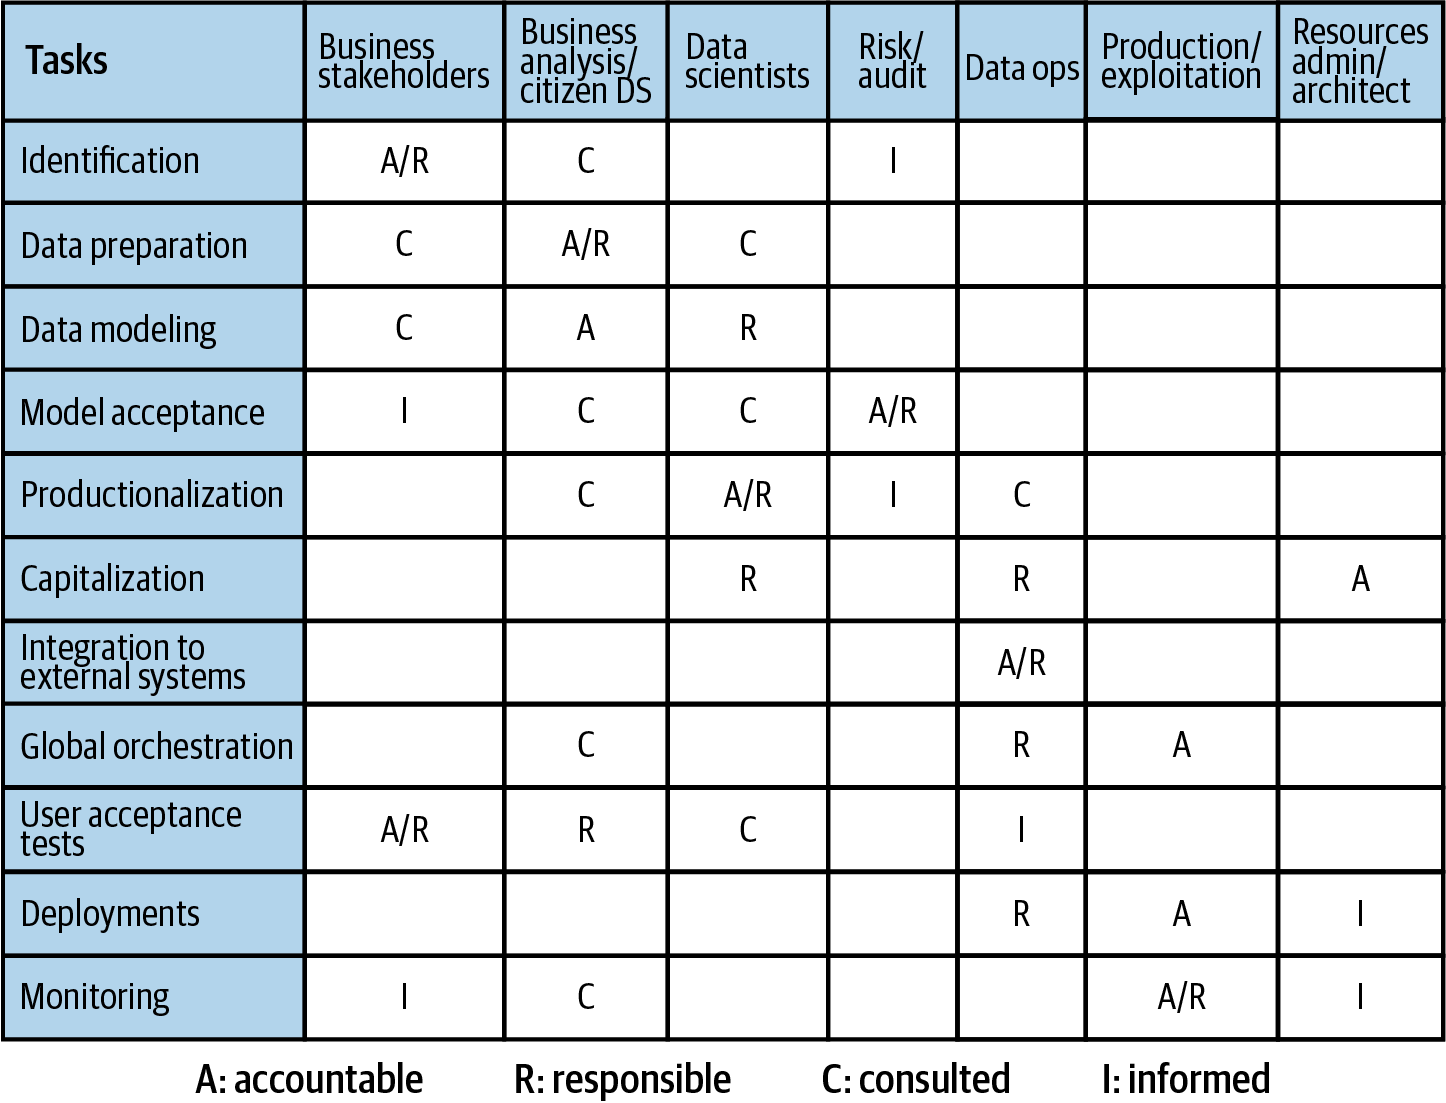
\includegraphics[height=2in]{imlo_0806.png} 
\end{column}
\begin{column}{.2\textwidth}
\tiny \textbf{Source:} Treveil et al. (2020), Figure 8-4
\end{column}
\end{columns}
\end{block}
\end{frame}

\begin{frame}{MLOps Governance \small [cont'd]}
\footnotesize
\begin{block}{4. Define Policies (''How will we do this?'')}
Establish rules for:
\begin{itemize}
   \item Reproducibility and traceability
   \item Auditability and documentation
   \item Sign-off between stages
   \item Model verification
   \item Model explainability
   \item Model bias and bias testing
   \item Model deployment mechanisms
   \item Model monitoring
   \item Data quality and data compliance
\end{itemize}
\end{block}
\tiny Adapted from Treveil et al. (2020), Chapter 8
\end{frame}

\begin{frame}{MLOps Governance \small [cont'd]}
\footnotesize
\begin{block}{5. Integrate Policies into MLOps Process (''When will we do this?'')}
\begin{itemize}
   \item Formalize and automate MLOps processes
   \item Define controls
   \item Define monitoring of controls
\end{itemize}
\end{block}

\begin{block}{6. Implement Governance Tools}
\begin{itemize}
   \item Automate controls
   \item Logging of control violations
   \item Auditing of control effectiveness
   \item Policy and procedure maintenance
\end{itemize}
\end{block}
\end{frame}

\begin{frame}{MLOps Governance \small [cont'd]}
\footnotesize
\begin{block}{7. Engage and Educate}
\begin{itemize}
   \item Communicate
   \item Awareness
   \item Training
   \item Buy-in \& commitment
   \item Culture
\end{itemize}
\end{block}

\begin{block}{8. Monitor and Refine}
\begin{itemize}
   \item Evaluate risk exposure
   \item Evaluate policy adequacy
   \item Evaluate control effectiveness
   \item Evaluate MLOps process performance
\end{itemize}
\end{block}
\end{frame}

\end{document}
